\PassOptionsToPackage{table}{xcolor}
\documentclass[aspectratio=169,11pt]{beamer}

% ── Theme ─────────────────────────────────────────────────────────────────────
\usetheme{metropolis}
\usepackage{appendixnumberbeamer}

% ── Packages ──────────────────────────────────────────────────────────────────
\usepackage[utf8]{inputenc}
\usepackage[T1]{fontenc}
\usepackage{amsmath,amssymb}
\usepackage{booktabs}
\usepackage{graphicx}
\usepackage{listings}
\usepackage{xcolor}
\usepackage{tikz}
\usetikzlibrary{positioning}
\usepackage{array}
\usepackage{multirow}

\lstset{
  basicstyle=\ttfamily\scriptsize,
  breaklines=true,
  frame=none,
  backgroundcolor=\color{gray!10},
  keywordstyle=\color{blue!70!black},
  commentstyle=\color{green!50!black}\itshape,
  stringstyle=\color{red!60!black},
}

\newcommand{\pres}[2]{\langle #1 \mid #2 \rangle}
\newcommand{\inv}[1]{#1^{-1}}

% ── Colours ───────────────────────────────────────────────────────────────────
\definecolor{good}{HTML}{2E7D32}
\definecolor{bad}{HTML}{C62828}
\definecolor{accent}{HTML}{1565C0}
\definecolor{highlight}{HTML}{FFF9C4}
\definecolor{neutral}{HTML}{F57F17}

% ── Title ─────────────────────────────────────────────────────────────────────
\title{Mini Reproduction Experiment:\\Diagnosing PPO on Andrews--Curtis}
\subtitle{Scaled-Down Ablation Study --- 147 Instances, 10M Steps, Run 2 Breakthrough}
\author{AC-Solver Project}
\date{April 2026}

\begin{document}

% ══════════════════════════════════════════════════════════════════════════════
\maketitle

% ══════════════════════════════════════════════════════════════════════════════
\begin{frame}{Outline}
  \tableofcontents
\end{frame}

% ══════════════════════════════════════════════════════════════════════════════
\section{Motivation: Why a Mini Experiment?}
% ══════════════════════════════════════════════════════════════════════════════

% ──────────────────────────────────────────────────────────────────────────────
\begin{frame}{The Problem: PPO vs.\ Paper Results}
  Our full-scale reproduction (100M steps, 1190 instances) showed:

  \begin{center}
  \begin{tabular}{lrrl}
    \toprule
    \textbf{Algorithm} & \textbf{Solved} & \textbf{Rate} & \textbf{Paper} \\
    \midrule
    Greedy ($10^6$ nodes)     & \textbf{554} / 1190 & 46.6\% & 533 (44.8\%) \\
    BFS ($10^6$ nodes)        & 278 / 1190           & 23.4\% & 278 (23.4\%) \\
    PPO (best-of-5, 50M)      & \textcolor{bad}{32} / 1190 & \textcolor{bad}{2.7\%} & \textcolor{good}{431 (36.2\%)} \\
    \bottomrule
  \end{tabular}
  \end{center}

  \bigskip
  \textbf{Classical search:} reproduced (BFS exact, greedy $+$21).\\
  \textbf{PPO:} $13\times$ gap.  \alert{Why?}

  \bigskip
  \textbf{Goal:} Identify the root cause(s) efficiently, without another 60-hour run.
\end{frame}

% ──────────────────────────────────────────────────────────────────────────────
\begin{frame}{Mini Experiment Design Philosophy}
  \begin{columns}[T]
    \begin{column}{0.48\textwidth}
      \textbf{Full experiment:}
      \begin{itemize}
        \item 1190 instances
        \item 100M steps ($\sim$60\,h)
        \item 1 configuration tested
        \item 1 data point
      \end{itemize}
    \end{column}
    \begin{column}{0.48\textwidth}
      \textbf{Mini experiment:}
      \begin{itemize}
        \item \textcolor{accent}{\textbf{147 instances}} (12.4\%)
        \item \textcolor{accent}{\textbf{10M steps}} ($\sim$6\,h each)
        \item \textcolor{accent}{\textbf{3 configurations}} tested
        \item 3 data points, controlled comparisons
      \end{itemize}
    \end{column}
  \end{columns}

  \bigskip
  \begin{block}{Key Insight}
    3 runs $\times$ 10M steps $=$ 30M total steps $=$ cost of less than half a single full run.\\
    We get 3 controlled comparisons instead of 1 expensive data point.
  \end{block}

  \bigskip
  Spec: \texttt{spec/2026-04-03-scaled-experiment.md}
\end{frame}

% ══════════════════════════════════════════════════════════════════════════════
\section{Systematic Diagnosis}
% ══════════════════════════════════════════════════════════════════════════════

% ──────────────────────────────────────────────────────────────────────────────
\begin{frame}{Root Causes, Ranked by Empirical Impact}
  \footnotesize
  \begin{center}
  \begin{tabular}{clll}
    \toprule
    \textbf{\#} & \textbf{Cause} & \textbf{Impact} & \textbf{Evidence} \\
    \midrule
    1 & \alert{\texttt{update\_epochs}${}=1$} & Single data pass & \textbf{Run 2 breakthrough} \\
    2 & Reward $\div 14{,}400$ & $+1000 \to +0.069$ & Not in paper \S4.3 \\
    3 & Batch $3.5\times$ smaller  & Noisier gradients  & 8 envs vs.\ 28 \\
    4 & No variable horizon        & Can't solve long-path & Paper: $200 \to 1200$ \\
    \bottomrule
  \end{tabular}
  \end{center}

  \bigskip
  \textbf{Primary finding:} \texttt{update\_epochs=4} was the critical fix.
  Run 2 (reward fix $+$ epochs${}=4$) solved \textbf{8/147 deterministic} and \textbf{10/147 stochastic}
  at 10M steps --- while Runs 0 and 1 (epochs${}=1$) solved 0 deterministic each.

  \bigskip
  \textbf{Secondary:} The reward fix improved the critic (expl.\ var $-1.7 \to 0.0$)
  but did \emph{not} improve the policy by itself (Run 1 $\approx$ Run 0 in evaluation).
\end{frame}

% ──────────────────────────────────────────────────────────────────────────────
\begin{frame}{Terminology: Deterministic vs.\ Stochastic Evaluation}
  \small
  After training, we evaluate the learned policy in two modes:

  \medskip
  \textbf{Deterministic (argmax):}
  \begin{itemize}\setlength\itemsep{2pt}
    \item At each step, choose the action with the \textbf{highest probability}:
      $a_t = \arg\max_a \pi_\theta(a \mid s_t)$
    \item Tests what the policy \emph{learned} --- its ``best guess'' at each state
    \item \textbf{Reproducible}: same state always produces the same action
    \item Strictest test of policy quality
  \end{itemize}

  \medskip
  \textbf{Stochastic (best-of-$k$):}
  \begin{itemize}\setlength\itemsep{2pt}
    \item Sample actions from the probability distribution:
      $a_t \sim \pi_\theta(\cdot \mid s_t)$
    \item Run $k$ independent rollouts per instance, report the best result
    \item Allows the policy to \textbf{explore} alternatives via randomness
    \item More forgiving: can ``get lucky'' on a good trajectory
  \end{itemize}

  \medskip
  \begin{block}{In Our Experiments}
    We evaluate at both: \textbf{deterministic} (det) and \textbf{stochastic best-of-5} (sto$\times$5).\\
    A policy that solves instances deterministically has learned \emph{genuine} structure.\\
    Stochastic-only solves may just be random walks that occasionally succeed.
  \end{block}
\end{frame}

% ──────────────────────────────────────────────────────────────────────────────
\begin{frame}{The Reward Attenuation Problem}
  \small
  The paper defines (Section~4.3):
  \[
    R(s_t, a_t, s_{t+1}) = \begin{cases}
      -\min(10,\; \mathrm{length}(s_{t+1})) & \text{if } \mathrm{length}(s_{t+1}) > 2 \\
      +1000 & \text{otherwise (solved)}
    \end{cases}
  \]

  \textbf{No further normalisation.}  PPO sees rewards in $[-10, +1000]$.

  \medskip
  Our code adds \alert{one extra line not in the paper}:
  \[
    \text{rewards} \;\mathrel{/}= \;\texttt{max\_reward} = 14{,}400
    \qquad\Longrightarrow\qquad
    \text{PPO sees } [-0.0007,\; +0.069]
  \]

  \begin{center}
    \begin{tabular}{lrr}
      \toprule
      & \textbf{Paper} & \textbf{Our code} \\
      \midrule
      Success reward     & $+1000$  & $+0.069$ \\
      Per-step penalty   & $-10$    & $-0.0007$ \\
      \textbf{Ratio}     & $100\times$ & $100\times$ \\
      \textbf{Magnitude} & \textcolor{good}{Large} & \textcolor{bad}{$14{,}400\times$ smaller} \\
      \bottomrule
    \end{tabular}
  \end{center}

  \smallskip
  {\scriptsize The \emph{ratio} is preserved, but the \emph{absolute magnitude} matters:
  with $\gamma=0.999$, a return of $0.062$ at step 100 is indistinguishable from noise.}
\end{frame}

% ──────────────────────────────────────────────────────────────────────────────
\begin{frame}{Worked Example: Why Normalisation Was Added (and Why It's Wrong)}
  \small
  The \texttt{max\_reward} constant comes from the environment's maximum possible
  single-step reward:
  \[
    \texttt{max\_reward} = T \times \texttt{max\_relator\_length} \times 2
    = 200 \times 36 \times 2 = 14{,}400
  \]
  This is the theoretical maximum return if \emph{every step gave the highest reward}.
  It was intended to normalise returns to $[0, 1]$ --- a common RL practice.

  \medskip
  \textbf{The problem:} The actual reward range is $[-10, +1000]$ (after clipping),
  not $[0, +14{,}400]$.  The normalisation constant was derived from the
  \emph{un-clipped} reward scale, but the code also applies clipping:

  \medskip
  \begin{center}
  \footnotesize
  \begin{tabular}{lrrl}
    \toprule
    \textbf{Stage} & \textbf{Success} & \textbf{Per-step} & \textbf{Code} \\
    \midrule
    1. Raw reward & $+14{,}400$ & $-10$ & \texttt{ACEnv.step()} \\
    2. Clip $[-10, 1000]$ & $+1{,}000$ & $-10$ & \texttt{clip\_rewards=True} \\
    3. $\div 14{,}400$ & $+0.069$ & $-0.0007$ & \texttt{rewards /= max\_reward} \\
    \bottomrule
  \end{tabular}
  \end{center}

  \medskip
  \textbf{Step 2 discards 93\% of the signal} ($14{,}400 \to 1{,}000$).\\
  \textbf{Step 3 then divides by a constant calibrated to the pre-clipped range},
  producing values $14.4\times$ smaller than intended.\\[3pt]
  The paper applies \textbf{only step 2}. Step 3 is our code's addition.
\end{frame}

% ──────────────────────────────────────────────────────────────────────────────
\begin{frame}{Worked Example: A Concrete Trajectory}
  \small
  Consider an episode where the agent solves a presentation at step $t = 80$:

  \medskip
  \textbf{Rewards along the trajectory} (presentation length decreasing from 12 to 2):
  \[
    r_0 = -10,\; r_1 = -10,\; \ldots,\; r_{79} = -8,\; r_{80} = +1000
  \]

  \textbf{Cumulative return} (from step 0, with $\gamma = 0.999$):
  \[
    G_0 = \sum_{t=0}^{80} \gamma^t r_t
    \approx \underbrace{-10 \cdot \frac{1 - 0.999^{80}}{1 - 0.999}}_{\text{penalties} \approx -770}
    + \underbrace{0.999^{80} \cdot 1000}_{\text{success} \approx +923}
    \approx +153
  \]

  \medskip
  \begin{center}
  \begin{tabular}{lrr}
    \toprule
    & \textbf{Paper scale} & \textbf{After $\div 14{,}400$} \\
    \midrule
    $G_0$ (step 0) & $+153$ & $+0.0106$ \\
    $G_{79}$ (step 79) & $+992$ & $+0.0689$ \\
    Unsolved trajectory $G_0$ & $-1{,}993$ & $-0.138$ \\
    \midrule
    \textbf{Spread} & $\sim 3{,}000$ & $\sim 0.2$ \\
    \bottomrule
  \end{tabular}
  \end{center}

  \smallskip
  With paper scale, the \textbf{critic} (a neural network that estimates future returns --- see frame~20)
  must distinguish returns differing by $\sim$3{,}000.\\
  After $\div 14{,}400$, all returns are within $\pm 0.14$ --- nearly flat.
\end{frame}

% ──────────────────────────────────────────────────────────────────────────────
\begin{frame}{Quantifying the Signal Loss}
  With $\gamma = 0.999$ and a success at step $t$:

  \smallskip
  \begin{center}
  \small
  \begin{tabular}{lrrl}
    \toprule
    & \textbf{Paper} & \textbf{Our code} & \textbf{Interpretation} \\
    \midrule
    Raw return at $t{=}0$   & $+1000$   & $+0.069$    & \\
    Discounted at $t{=}50$  & $+951$    & $+0.066$    & Still strong vs.\ still tiny \\
    Discounted at $t{=}100$ & $+905$    & $+0.063$    & Clear signal vs.\ noise \\
    \midrule
    Per-step penalty         & $-10$     & $-0.0007$   & \\
    SNR at $t{=}100$         & $\sim 90$ & $\sim 90$   & Ratio same, scale not \\
    \midrule
    Critic init scale       & \multicolumn{2}{c}{$O(1)$} & Ortho init, gain${}=1.0$ \\
    Critic target           & $O(1000)$ & $O(0.07)$    & \textcolor{bad}{Critic already ``accurate''} \\
    \bottomrule
  \end{tabular}
  \end{center}

  \medskip
  \textbf{Key insight:} PPO trains a \textbf{critic} network to predict future returns from each state
  (details in the PPO section).
  The critic's random initial predictions are $O(1)$, which is
  already $14\times$ the actual returns.  The critic has no gradient signal to improve
  because its MSE loss is dominated by the initialisation scale, not the reward signal.
\end{frame}

% ══════════════════════════════════════════════════════════════════════════════
\section{PPO Algorithm Review}
% ══════════════════════════════════════════════════════════════════════════════

% ──────────────────────────────────────────────────────────────────────────────
\begin{frame}{Step 1: The RL Loop as a Markov Decision Process}
  \small
  We cast AC-trivialization as an MDP $(S, A, R, P, \rho)$:

  \medskip
  \begin{center}
  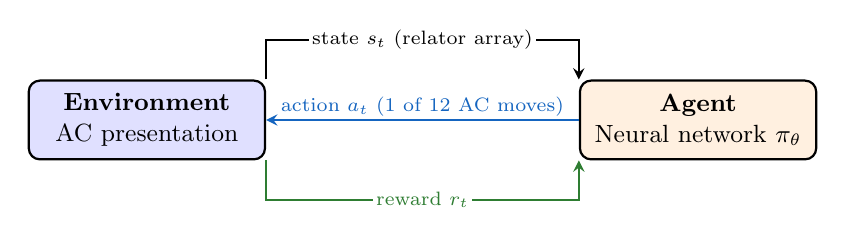
\begin{tikzpicture}[
    box/.style={draw, rounded corners, minimum height=1cm, minimum width=3cm,
                align=center, font=\small, thick},
    arrow/.style={->, thick, >=stealth},
    lbl/.style={font=\scriptsize, fill=white, inner sep=1pt}
  ]
    \node[box, fill=blue!12] (env) at (0,0) {\textbf{Environment}\\AC presentation};
    \node[box, fill=orange!12] (agent) at (7,0) {\textbf{Agent}\\Neural network $\pi_\theta$};

    \draw[arrow] (env.north east) -- ++(0,0.5) -| node[lbl, pos=0.25] {state $s_t$ (relator array)} (agent.north west);
    \draw[arrow, color=good] (env.south east) -- ++(0,-0.5) -| node[lbl, pos=0.25] {reward $r_t$} (agent.south west);
    \draw[arrow, color=accent] (agent.west) -- node[lbl, above] {action $a_t$ (1 of 12 AC moves)} (env.east);
  \end{tikzpicture}
  \end{center}

  \begin{itemize}\setlength\itemsep{2pt}
    \item \textbf{State} $s_t$: a balanced presentation $\pres{x,y}{r_0, r_1}$ encoded as an integer array
    \item \textbf{Action} $a_t \in \{0, \ldots, 11\}$: one of 12 AC moves (see next slide)
    \item \textbf{Reward} $r_t = R(s_t, a_t, s_{t+1})$: depends on the resulting presentation length
    \item \textbf{Goal}: find a policy $\pi_\theta$ that maximizes cumulative return:
  \end{itemize}
  \vspace{-4pt}
  \[
    R(\tau) = \sum_{t=0}^{T} \gamma^t\, R(s_t, a_t, s_{t+1}),
    \qquad \gamma = 0.999
  \]
\end{frame}

% ──────────────────────────────────────────────────────────────────────────────
\begin{frame}{The 12 AC Moves (Action Space)}
  \footnotesize
  The original AC moves (Section~2 of the paper) are:
  \begin{itemize}\setlength\itemsep{0pt}
    \item[(AC1)] $r_i \to r_i r_j^{\pm 1}$ for $i \neq j$ \quad (concatenation)
    \item[(AC2)] $r_i \to \inv{r_i}$ \quad (inversion --- \alert{dropped}: doesn't change length $\Rightarrow$ no signal)
    \item[(AC3)] $r_i \to g\, r_i\, \inv{g}$ where $g$ is a generator or its inverse \quad (conjugation)
  \end{itemize}

  \smallskip
  The number of moves depends on the number of \textbf{generators} $n_g$ and \textbf{relators} $n_r$:
  \[
    |\text{AC moves}| = \underbrace{n_r(n_r - 1) \cdot 2}_{\text{AC'1: concatenations}}
    + \underbrace{n_r \cdot 2 n_g}_{\text{AC'2: conjugations}}
    = 2n_r(n_r - 1) + 2 n_r n_g
  \]
  For our setting ($n_g = 2$ generators $\{x, y\}$, $n_r = 2$ relators $\{r_0, r_1\}$):
  $= 2 \cdot 2 \cdot 1 + 2 \cdot 2 \cdot 2 = 4 + 8 = \mathbf{12}$ moves.

  \smallskip
  {\scriptsize \textbf{Note:} The paper (p7) states ``$3n^2$ AC moves'' for $n$ generators.
  With $n = 2$: $3 \cdot 4 = 12$, consistent. For a 3-generator problem, this would
  be $3 \cdot 9 = 27$ moves --- the action space grows quadratically.}

\end{frame}

% ──────────────────────────────────────────────────────────────────────────────
\begin{frame}{The 12 AC Moves: Concatenations and Conjugations}
  \footnotesize
  \begin{columns}[T]
    \begin{column}{0.44\textwidth}
      \textbf{Concatenations} (4 moves)\\[2pt]
      \scriptsize
      \begin{tabular}{cl}
        \toprule
        \textbf{ID} & \textbf{Move} \\
        \midrule
        0 & $r_1 \to r_1 \cdot r_0$ \\
        1 & $r_0 \to r_0 \cdot \inv{r_1}$ \\
        2 & $r_1 \to r_1 \cdot \inv{r_0}$ \\
        3 & $r_0 \to r_0 \cdot r_1$ \\
        \bottomrule
      \end{tabular}
    \end{column}
    \begin{column}{0.54\textwidth}
      \textbf{Conjugations} (8 moves)\\[2pt]
      \scriptsize
      \begin{tabular}{cl}
        \toprule
        \textbf{ID} & \textbf{Move} \\
        \midrule
        4  & $r_1 \to \inv{x}\, r_1\, x$ \\
        5  & $r_0 \to \inv{y}\, r_0\, y$ \\
        6  & $r_1 \to \inv{y}\, r_1\, y$ \\
        7  & $r_0 \to x\, r_0\, \inv{x}$ \\
        8  & $r_1 \to x\, r_1\, \inv{x}$ \\
        9  & $r_0 \to y\, r_0\, \inv{y}$ \\
        10 & $r_1 \to y\, r_1\, \inv{y}$ \\
        11 & $r_0 \to \inv{x}\, r_0\, x$ \\
        \bottomrule
      \end{tabular}
    \end{column}
  \end{columns}

  \bigskip
  \begin{itemize}\setlength\itemsep{2pt}
    \item After each move, \textbf{free reduction} cancels adjacent inverse pairs
      (e.g., $x\inv{x} \to \varepsilon$).
    \item \textbf{Cyclic reduction} cancels at word boundaries (equivalent to conjugation).
    \item If a move would exceed \texttt{max\_relator\_length} $= 36$, it is \textbf{rejected}
      (a ``no-op'' --- the state is returned unchanged).
    \item In practice, $\sim$60--70\% of actions are no-ops (many moves violate the length bound).
  \end{itemize}
\end{frame}

% ──────────────────────────────────────────────────────────────────────────────
\begin{frame}{Step 2a: The Policy Gradient Theorem}
  \small
  \textbf{Policy} $\pi_\theta(a \mid s)$: a neural network that outputs a probability distribution
  over the 12 AC moves, given a presentation state $s$.

  \medskip
  \textbf{Goal:} find $\theta$ that maximises the expected return $J(\pi_\theta) = \mathbb{E}_{\tau \sim \pi_\theta}[R(\tau)]$.

  \medskip
  \textbf{The Policy Gradient Theorem} (Williams 1992, Sutton et al.\ 1999) shows:
  \[
    \nabla_\theta J(\pi_\theta) = \mathbb{E}_{\tau \sim \pi_\theta}\!\left[
      \sum_{t=0}^{T} \nabla_\theta \log \pi_\theta(a_t \mid s_t)\; A^{\pi}(s_t, a_t)
    \right]
  \]

  Two key terms:
  \begin{itemize}\setlength\itemsep{2pt}
    \item $\nabla_\theta \log \pi_\theta(a_t \mid s_t)$: the \textbf{score function} ---
      the direction in parameter space that makes action $a_t$ more likely from state $s_t$.
    \item $A^{\pi}(s_t, a_t)$: the \textbf{advantage} --- ``how much better was action $a_t$
      compared to the \emph{average} action from state $s_t$?''
  \end{itemize}

  \medskip
  \textbf{Vanilla policy gradient} directly optimises:
  \[
    L^{PG} = \mathbb{E}_t\!\left[
      \log \pi_\theta(a_t \mid s_t)\; A^{\pi}(s_t, a_t)
    \right]
  \]
  This increases the probability of actions with positive advantage and decreases
  the probability of actions with negative advantage.
\end{frame}

% ──────────────────────────────────────────────────────────────────────────────
\begin{frame}{Step 2b: Why Vanilla Policy Gradient Fails}
  \small
  \textbf{Problem:} vanilla policy gradient can make \textbf{catastrophically large updates}.

  \medskip
  \textbf{Concrete example from our AC problem:}

  \smallskip
  Suppose the current policy gives move~3 (concatenation $r_0 \to r_0 r_1$)
  probability $\pi(a_3 \mid s) = 0.10$ (roughly uniform across 12 moves).
  The advantage estimate says this move was very good: $A = +5$.

  \medskip
  A single gradient step on $L^{PG} = \log(0.10) \times 5 = -11.5$ pushes $\theta$
  to increase $\pi(a_3 \mid s)$. With a large learning rate, one step might give:
  \[
    \pi(a_3 \mid s): \quad 0.10 \;\to\; 0.85
  \]

  \textbf{What if the advantage estimate was wrong?}
  (Noisy critic, small batch, early training --- all common.)
  The policy now confidently chooses move~3 from state $s$
  and may \textbf{never explore alternatives}, leading to permanent failure.
\end{frame}

% ──────────────────────────────────────────────────────────────────────────────
\begin{frame}{Step 2c: Three Approaches to Constraining Updates}
  \small
  The core problem: the gradient $\nabla_\theta L^{PG}$ tells us a \emph{direction}
  to improve, but gives no guidance on \emph{how far} to step.

  \medskip
  \textbf{Three approaches to constraining the step size:}

  \begin{enumerate}\setlength\itemsep{6pt}
    \item \textbf{Small learning rate:} simple but too conservative --- wastes
      data by making tiny updates even when larger ones are safe.

    \item \textbf{TRPO} (Schulman et al., 2015): constrain the KL divergence
      $D_{KL}(\pi_\text{old} \| \pi_\theta) \le \delta$ after each update.
      Effective but requires expensive second-order optimisation (conjugate gradient).

    \item \textbf{PPO} (Schulman et al., 2017): \alert{clip the probability ratio}
      $r_t = \pi_\theta / \pi_\text{old}$ to $[1{-}\epsilon,\; 1{+}\epsilon]$
      \emph{inside} the objective.  First-order only, simple to implement.
  \end{enumerate}

  \bigskip
  \textbf{Our paper uses PPO} --- the simplest and most widely adopted approach.
  The next frames explain how the clipping mechanism works.
\end{frame}

% ──────────────────────────────────────────────────────────────────────────────
\begin{frame}{Step 2d: Why PPO Clipping Enables Multiple Epochs}
  \small
  \begin{block}{PPO's Key Insight}
    By clipping the probability ratio at $\epsilon = 0.2$, the policy can only change by
    $\pm 20\%$ per update.
  \end{block}

  \medskip
  This has three important consequences:

  \begin{enumerate}\setlength\itemsep{6pt}
    \item \textbf{Conservative enough} to prevent catastrophic collapses ---
      even with a noisy advantage estimate, one bad gradient step can only
      shift probabilities by 20\%, not from 10\% to 90\%.

    \item \textbf{Permissive enough} to allow steady learning ---
      over many updates, the policy can still change dramatically
      (20\% per step compounds quickly).

    \item \textbf{Safe for multiple epochs} --- since each pass over the batch
      can only move the policy $\pm 20\%$, reusing the same batch 4 times
      won't cause divergence.  This is \alert{critical for our fix}: it's what
      makes \texttt{epochs=4} safe despite the small batch size.
  \end{enumerate}

  \medskip
  Without clipping, multiple epochs would overfit to the batch ---
  the policy would chase noisy advantages until it collapsed.
\end{frame}

% ──────────────────────────────────────────────────────────────────────────────
\begin{frame}{Step 3a: The Probability Ratio}
  \small
  PPO reformulates the policy gradient using the \textbf{probability ratio}:
  \[
    r_t(\theta) = \frac{\pi_\theta(a_t \mid s_t)}{\pi_{\theta_\text{old}}(a_t \mid s_t)}
  \]

  \textbf{Interpretation:}
  \begin{itemize}\setlength\itemsep{2pt}
    \item $r_t = 1$: the new policy assigns the \emph{same} probability to action $a_t$
      from state $s_t$ as the old policy. No change.
    \item $r_t = 1.5$: the new policy is 50\% \emph{more} likely to take this action.
    \item $r_t = 0.7$: the new policy is 30\% \emph{less} likely to take this action.
  \end{itemize}

  \medskip
  \textbf{Why use a ratio?}  The vanilla gradient uses $\log \pi_\theta(a \mid s)$,
  which can produce arbitrarily large updates.  The ratio $r_t$ lets us directly
  measure ``how much did the policy change?'' and \textbf{limit it}.

  \medskip
  \textbf{Importance sampling:} Since we collected data under $\pi_\text{old}$ but want
  to improve $\pi_\theta$, the ratio corrects for this mismatch:
  \[
    L^{IS}(\theta) = \mathbb{E}_{a_t \sim \pi_\text{old}}\!\left[
      r_t(\theta)\, A_t
    \right]
    = \mathbb{E}_{a_t \sim \pi_\theta}\!\left[ A_t \right]
  \]
  This is mathematically equivalent to the vanilla gradient but expressed in terms of the ratio.
\end{frame}

% ──────────────────────────────────────────────────────────────────────────────
\begin{frame}{Step 3b: The Clipped Surrogate Objective}
  \small
  The unconstrained objective $L^{IS} = \mathbb{E}[r_t A_t]$ can still produce large updates
  (if $r_t$ becomes very large).  PPO \textbf{clips} the ratio:
  \[
    L^{CLIP}(\theta) = \mathbb{E}_t\!\Big[
      \min\!\big( r_t(\theta)\, A_t,\;
      \mathrm{clip}(r_t(\theta),\, 1{-}\epsilon,\, 1{+}\epsilon)\, A_t \big)
    \Big],
    \qquad \epsilon = 0.2
  \]

  \textbf{Reading this equation:}
  \begin{itemize}\setlength\itemsep{3pt}
    \item $r_t(\theta) A_t$: the \textbf{unclipped} objective --- how much the policy improves
    \item $\mathrm{clip}(r_t, 0.8, 1.2) \cdot A_t$: the \textbf{clipped} version ---
      caps the ratio so the policy can change by at most $\pm 20\%$
    \item $\min(\cdot, \cdot)$: take whichever gives a \textbf{smaller improvement}
      (the ``pessimistic bound'')
  \end{itemize}

  \medskip
  \textbf{Why $\min$?}  We want to be \emph{conservative}: if the unclipped objective
  says ``increase this action's probability by 50\%'' but the clipped version says
  ``only allow 20\%'', we use the clipped (smaller) version.
\end{frame}

% ──────────────────────────────────────────────────────────────────────────────
\begin{frame}{Step 3c: Clipping --- Case-by-Case Analysis}
  \small
  \begin{tabular}{lp{9.5cm}}
    \toprule
    \textbf{Case} & \textbf{What happens} \\
    \midrule
    $A_t > 0$, $r_t < 1.2$ & Unclipped: gradient encourages increasing $\pi(a_t \mid s_t)$ normally \\[3pt]
    $A_t > 0$, $r_t \ge 1.2$ & \textbf{Clipped}: $r_t$ capped at 1.2. No further gradient to increase probability beyond 20\% \\[3pt]
    $A_t < 0$, $r_t > 0.8$ & Unclipped: gradient encourages decreasing $\pi(a_t \mid s_t)$ normally \\[3pt]
    $A_t < 0$, $r_t \le 0.8$ & \textbf{Clipped}: $r_t$ floored at 0.8. No further gradient to decrease beyond 20\% \\
    \bottomrule
  \end{tabular}

  \bigskip
  \textbf{Intuition:}
  \begin{itemize}\setlength\itemsep{3pt}
    \item \textbf{Good action} ($A_t > 0$): we want to increase its probability, but not
      too fast $\Rightarrow$ cap at $+20\%$.
    \item \textbf{Bad action} ($A_t < 0$): we want to decrease its probability, but not
      too fast $\Rightarrow$ floor at $-20\%$.
    \item In both cases, once the clip activates, \textbf{the gradient is zero} ---
      no further update is applied for that transition.
  \end{itemize}

  \medskip
  This is what makes PPO safe for multiple epochs: each pass can only move the policy
  by $\pm 20\%$, preventing runaway divergence from the rollout policy.
\end{frame}

% ──────────────────────────────────────────────────────────────────────────────
\begin{frame}[fragile]{PPO Clipping: In Our Code}
  \small
  The actual implementation in \texttt{training.py} (lines 386--415):

  \begin{lstlisting}[language=python]
logratio = newlogprob - b_logprobs[mb_inds]
ratio = logratio.exp()  # pi(a|s) / pi_old(a|s)

# Advantage normalisation (scale-invariant!)
mb_advantages = (mb_advantages - mb_advantages.mean()) / (
    mb_advantages.std() + 1e-8)

# Clipped policy loss
pg_loss1 = -mb_advantages * ratio
pg_loss2 = -mb_advantages * torch.clamp(
    ratio, 1 - clip_coef, 1 + clip_coef)     # clip_coef = 0.2
pg_loss = torch.max(pg_loss1, pg_loss2).mean()
  \end{lstlisting}

\end{frame}

% ──────────────────────────────────────────────────────────────────────────────
\begin{frame}{PPO Clipping: A Numerical Example}
  \small
  \textbf{One transition from our AC problem:}
  \begin{center}
  \begin{tabular}{lrl}
    \toprule
    \textbf{Quantity} & \textbf{Value} & \textbf{Meaning} \\
    \midrule
    $\pi_\text{old}(a_3 \mid s)$ & 0.10 & Old policy: move~3 had 10\% probability \\
    $\pi_\text{new}(a_3 \mid s)$ & 0.15 & After gradient step: now 15\% \\
    $r_t = 0.15 / 0.10$ & 1.50 & 50\% increase --- too much! \\
    $\mathrm{clip}(r_t, 0.8, 1.2)$ & \textbf{1.20} & Capped at 20\% increase \\
    \midrule
    $A_t > 0$ (good action) & & $\min(1.5 A_t,\; 1.2 A_t) = 1.2 A_t$ \\
    & & $\Rightarrow$ gradient only ``sees'' 20\% change \\
    \bottomrule
  \end{tabular}
  \end{center}

  \medskip
  \textbf{How \texttt{torch.max} implements the pessimistic bound:}
  \begin{itemize}\setlength\itemsep{2pt}
    \item The loss is \emph{negated}: \texttt{pg\_loss1 = -A * r}, \texttt{pg\_loss2 = -A * clip(r)}
    \item We \emph{minimise} the loss, so \texttt{torch.max(loss1, loss2)} picks the
      \emph{least negative} (= smallest improvement)
    \item This ensures the clipped version is used whenever it gives a more conservative update
    \item \textbf{Effect:} the policy can never ``overshoot'' by more than $\epsilon = 20\%$
      in a single gradient step
  \end{itemize}
\end{frame}

% ──────────────────────────────────────────────────────────────────────────────
\begin{frame}{Step 4: Actor-Critic Architecture}
  \small
  PPO trains \textbf{two separate networks} simultaneously:

  \medskip
  \begin{center}
  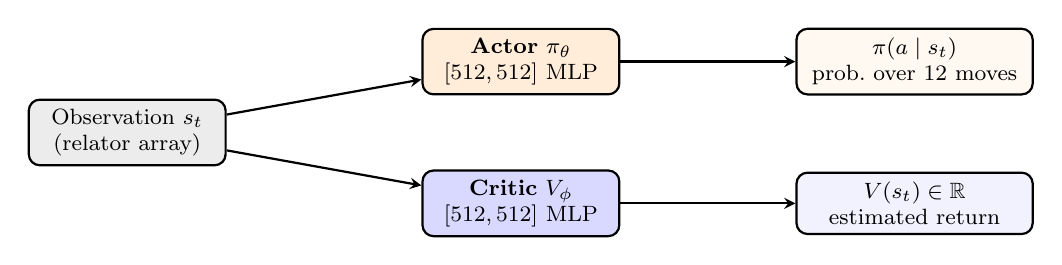
\begin{tikzpicture}[
    box/.style={draw, rounded corners, minimum height=0.7cm, minimum width=2.5cm,
                align=center, font=\footnotesize, thick},
    arrow/.style={->, thick, >=stealth},
  ]
    \node[box, fill=gray!15] (obs) at (0,0) {Observation $s_t$\\(relator array)};
    \node[box, fill=orange!15] (actor) at (5, 0.9) {\textbf{Actor} $\pi_\theta$\\$[512, 512]$ MLP};
    \node[box, fill=blue!15]   (critic) at (5,-0.9) {\textbf{Critic} $V_\phi$\\$[512, 512]$ MLP};
    \node[box, fill=orange!5, minimum width=3cm] (pi) at (10, 0.9) {$\pi(a \mid s_t)$\\prob.\ over 12 moves};
    \node[box, fill=blue!5, minimum width=3cm]   (val) at (10,-0.9) {$V(s_t) \in \mathbb{R}$\\estimated return};

    \draw[arrow] (obs) -- (actor);
    \draw[arrow] (obs) -- (critic);
    \draw[arrow] (actor) -- (pi);
    \draw[arrow] (critic) -- (val);
  \end{tikzpicture}
  \end{center}

  \medskip
  \begin{itemize}\setlength\itemsep{1pt}
    \item \textbf{Actor loss} $L^{CLIP}$: push policy toward actions with positive advantage
    \item \textbf{Critic loss} $L^V = \mathrm{MSE}\big(V_\phi(s_t),\; G_t\big)$: predict actual returns from each state
    \item \textbf{Entropy bonus} $H[\pi]$: prevents premature convergence to a single action
  \end{itemize}

  \smallskip
  \textbf{Entropy} $H[\pi]$ measures how ``spread out'' the policy's probability distribution is:
  \[
    H[\pi(\cdot \mid s_t)] = -\sum_{a=1}^{12} \pi(a \mid s_t) \log \pi(a \mid s_t)
  \]
  \vspace{-6pt}
  \begin{itemize}\setlength\itemsep{0pt}
    \item $H = 0$ when the policy is deterministic (all probability on one action)
    \item $H = \log 12 \approx 2.48$ when uniform over all 12 moves (maximum exploration)
  \end{itemize}

  \smallskip
  \textbf{Combined loss} (optimized jointly with a single Adam optimizer):
  \[
    \mathcal{L} = L^{CLIP}
    - \underbrace{c_\text{ent}}_{\scriptscriptstyle 0.01} \cdot H[\pi]
    + \underbrace{c_\text{vf}}_{\scriptscriptstyle 0.5} \cdot L^V
  \]
  The $-c_\text{ent}\cdot H[\pi]$ term \emph{rewards} high entropy, encouraging the agent to keep exploring.
\end{frame}

% ──────────────────────────────────────────────────────────────────────────────
\begin{frame}{Step 5: Rollout Phase --- Collecting a Batch}
  \small
  Before each PPO update, the agent collects data by running $N$ environments
  in parallel for $T$ steps each.

  \medskip
  \textbf{Definition:} A \textbf{batch} is the set of all transitions collected in one rollout:
  \[
    \text{batch\_size} = \underbrace{N}_{\text{envs}} \times \underbrace{T}_{\text{steps per env}}
  \]
  \vspace{-8pt}

  \begin{center}
  \scriptsize
  \begin{tabular}{p{1.3cm}p{10cm}}
    \toprule
    \textbf{Env 1} & $(s_0, a_0, r_0, s_1),\; (s_1, a_1, r_1, s_2),\; \ldots,\; (s_{199}, a_{199}, r_{199}, s_{200})$ \\
    \textbf{Env 2} & $(s_0, a_0, r_0, s_1),\; (s_1, a_1, r_1, s_2),\; \ldots$ \\
    $\vdots$ & $\vdots$ \\
    \textbf{Env $N$} & $(s_0, a_0, r_0, s_1),\; \ldots$ \\
    \bottomrule
  \end{tabular}
  \end{center}

  \smallskip
  Each row is an independent AC presentation explored simultaneously.
  Each transition records: state, action (which of 12 moves), reward, and next state.

  \medskip
  \textbf{Our numbers:} $N = 8$, $T = 200$ $\Rightarrow$ batch of \textbf{1{,}600 transitions}
  per update.  The paper uses $N = 28$ $\Rightarrow$ \textbf{5{,}600 transitions}.
\end{frame}

% ──────────────────────────────────────────────────────────────────────────────
\begin{frame}{Step 6: Computing Advantages with GAE}
  \small
  After collecting a batch, we compute \textbf{how good each action was}.

  \medskip
  \textbf{Advantage} $\hat{A}_t$: the difference between the actual return and what the critic predicted:
  \[
    \hat{A}_t = G_t - V(s_t)
    \quad\text{where}\quad
    G_t = \sum_{k=0}^{T-t} \gamma^k\, r_{t+k}
  \]
  \vspace{-6pt}

  \textbf{Generalized Advantage Estimation (GAE)} smooths this using parameter $\lambda$:
  \[
    \hat{A}_t^\text{GAE} = \sum_{k=0}^{T-t} (\gamma \lambda)^k \,\delta_{t+k},
    \qquad \delta_t = r_t + \gamma V(s_{t+1}) - V(s_t)
  \]
  \vspace{-6pt}

  \begin{itemize}\setlength\itemsep{1pt}
    \item $\lambda = 0$: one-step TD error only (low variance, high bias)
    \item $\lambda = 1$: full Monte Carlo return (high variance, low bias)
    \item \textbf{Our setting:} $\lambda = 0.95$ --- a standard compromise
  \end{itemize}

  \smallskip
  \textbf{Intuition:} $\delta_t$ asks ``was this step better or worse than the critic expected?''
  GAE averages these one-step judgments over the trajectory, exponentially down-weighting
  future steps.
\end{frame}

% ──────────────────────────────────────────────────────────────────────────────
\begin{frame}{Worked Example: Computing $G_t$ and $V(s_t)$}
  \small
  \textbf{Scenario:} An AC environment episode of 5 steps, with $\gamma = 0.99$.

  \medskip
  \textbf{Rewards received:} $r_0 = -1,\; r_1 = -1,\; r_2 = -1,\; r_3 = -1,\; r_4 = +1000$ (solved at step 4).

  \medskip
  \textbf{$G_t$ (actual discounted return)} is computed \emph{backwards} from the end:
  \begin{align*}
    G_4 &= r_4 = +1000 \\
    G_3 &= r_3 + \gamma G_4 = -1 + 0.99 \times 1000 = +989.0 \\
    G_2 &= r_2 + \gamma G_3 = -1 + 0.99 \times 989.0 = +978.11 \\
    G_1 &= r_1 + \gamma G_2 = -1 + 0.99 \times 978.11 = +967.33 \\
    G_0 &= r_0 + \gamma G_1 = -1 + 0.99 \times 967.33 = +956.66
  \end{align*}
  \vspace{-10pt}

  \textbf{$V(s_t)$ (critic's prediction)} is the neural network's \emph{guess} at $G_t$
  \emph{before} the episode unfolds.  Early in training, the critic is random:

  \medskip
  \begin{center}\footnotesize
  \begin{tabular}{lrrrl}
    \toprule
    $t$ & $G_t$ (actual) & $V(s_t)$ (critic) & $\hat{A}_t = G_t - V(s_t)$ & \textbf{Interpretation} \\
    \midrule
    0 & $+956.66$ & $+2.1$ & $+954.56$ & Action much better than expected \\
    3 & $+989.00$ & $-0.3$ & $+989.30$ & Critic had no idea this leads to solve \\
    \bottomrule
  \end{tabular}
  \end{center}

  \smallskip
  \textbf{Key:} $G_t$ uses the \emph{actual} rewards (known after rollout).
  $V(s_t)$ is the critic's estimate (updated by training on $L^V = (V(s_t) - G_t)^2$).
  Over time, $V(s_t) \to G_t$ and advantages shrink.
\end{frame}

% ──────────────────────────────────────────────────────────────────────────────
\begin{frame}{Step 7: The Full PPO Training Loop}
  \small
  Putting it all together --- training alternates between \textbf{collecting data} and \textbf{updating}:

  \medskip
  \begin{center}
  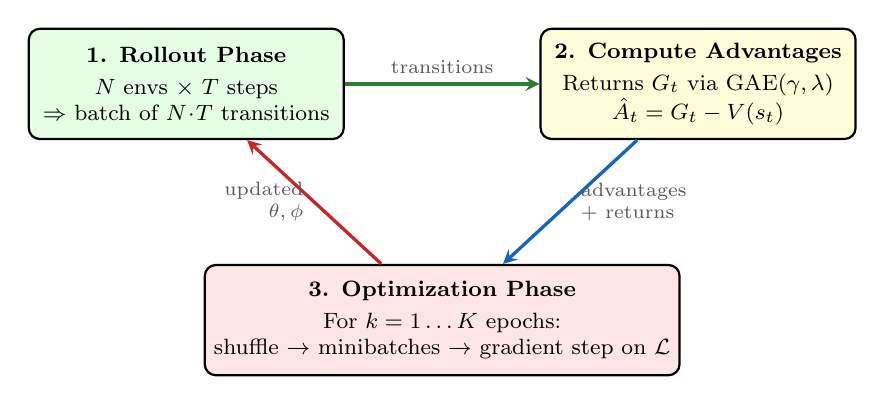
\begin{tikzpicture}[
    phase/.style={draw, rounded corners, minimum height=1.4cm, minimum width=4cm,
                  align=center, font=\footnotesize, thick},
    arrow/.style={->, very thick, >=stealth},
    steplbl/.style={font=\scriptsize, text=gray!70!black}
  ]
    \node[phase, fill=green!10] (rollout) at (0,0) {
      \textbf{1. Rollout Phase}\\[2pt]
      $N$ envs $\times$ $T$ steps\\
      $\Rightarrow$ batch of $N \!\cdot\! T$ transitions
    };
    \node[phase, fill=yellow!15] (gae) at (6.5,0) {
      \textbf{2. Compute Advantages}\\[2pt]
      Returns $G_t$ via GAE($\gamma, \lambda$)\\
      $\hat{A}_t = G_t - V(s_t)$
    };
    \node[phase, fill=red!10] (optim) at (3.25,-3) {
      \textbf{3. Optimization Phase}\\[2pt]
      For $k = 1 \ldots K$ epochs:\\
      shuffle $\to$ minibatches $\to$ gradient step on $\mathcal{L}$
    };

    \draw[arrow, color=good] (rollout) -- node[steplbl, above] {transitions} (gae);
    \draw[arrow, color=accent] (gae) -- node[steplbl, right, align=left] {advantages\\+ returns} (optim);
    \draw[arrow, color=bad] (optim) -- node[steplbl, left, align=right] {updated\\$\theta, \phi$} (rollout);
  \end{tikzpicture}
  \end{center}

  Each cycle around this loop is \textbf{one rollout} (= one batch of $N \!\cdot\! T$ transitions).
  Training repeats this loop until the total step budget is exhausted.
\end{frame}

% ──────────────────────────────────────────────────────────────────────────────
\begin{frame}{PPO Training Loop: How Many Rollouts in Our Case?}
  \small
  \textbf{In our case} ($N=8$ envs, $T=200$ steps, 10M total steps):

  \begin{itemize}\setlength\itemsep{3pt}
    \item Each rollout collects $8 \times 200 = 1{,}600$ transitions
    \item Total rollouts = $\dfrac{10{,}000{,}000}{1{,}600} = \textbf{6{,}250}$ cycles around the loop
    \item Each cycle:
      \begin{itemize}\setlength\itemsep{1pt}
        \item \textbf{Rollout phase:} $\sim$1.2s (run 8 envs for 200 steps each)
        \item \textbf{GAE computation:} $\sim$0.01s (backward pass over stored rewards)
        \item \textbf{Optimization:} $\sim$0.1s ($K{=}1$) or $\sim$0.4s ($K{=}4$)
      \end{itemize}
    \item Total wall-clock: $6{,}250 \times 1.6\text{s} \approx \textbf{2.8\,h}$ on Mac MPS
  \end{itemize}

  \medskip
  \textbf{Comparison with the paper} ($N=28$, $T=200$, 100M total steps):
  \begin{itemize}\setlength\itemsep{1pt}
    \item Each rollout: $28 \times 200 = 5{,}600$ transitions
    \item Total rollouts: $\frac{100{,}000{,}000}{5{,}600} = \textbf{17{,}857}$ cycles
    \item 3$\times$ more data per rollout, 3$\times$ more rollouts, and 10$\times$ more total steps
  \end{itemize}
\end{frame}

% ──────────────────────────────────────────────────────────────────────────────
\begin{frame}{PPO Training Loop: Hyperparameter Comparison}
  \small
  \textbf{Our setup vs.\ the paper:}
  \begin{center}
  \begin{tabular}{lrrl}
    \toprule
    \textbf{Quantity} & \textbf{Paper} & \textbf{Ours} & \textbf{Meaning} \\
    \midrule
    $N$ (parallel envs) & 28 & 8 & Simultaneous presentations \\
    $T$ (rollout length) & 200 & 200 & Steps per env before updating \\
    Batch size & 5{,}600 & 1{,}600 & Transitions per PPO update \\
    Minibatch size & 1{,}400 & 400 & Transitions per gradient step \\
    $K$ (epochs) & 1 & 1 or \textbf{4} & Passes over batch per update \\
    Total updates & 17{,}857 & 6{,}250 & In a 10M-step run \\
    \bottomrule
  \end{tabular}
  \end{center}

  \medskip
  \textbf{Key ratio:} The paper sees each transition once per update (epochs$=$1),
  but has $3.5\times$ more transitions per batch.
  With epochs$=$4, our effective data per update is $1{,}600 \times 4 = 6{,}400$,
  \emph{exceeding} the paper's 5{,}600.
\end{frame}

% ──────────────────────────────────────────────────────────────────────────────
\begin{frame}{PPO Training Loop: Timing Breakdown}
  \small
  \textbf{One PPO update cycle:}
  \begin{enumerate}\setlength\itemsep{4pt}
    \item \textbf{Rollout:} 8 envs $\times$ 200 steps $= 1{,}600$ transitions ($\sim$1.2s)
    \item \textbf{GAE:} compute advantages and returns ($\sim$0.01s)
    \item \textbf{Optimize:} $K$ epochs $\times$ 4 minibatches $\times$ 1 gradient step each
      \begin{itemize}\setlength\itemsep{1pt}
        \item $K{=}1$: $1 \times 4 = 4$ gradient steps ($\sim$0.1s)
        \item $K{=}4$: $4 \times 4 = 16$ gradient steps ($\sim$0.4s)
      \end{itemize}
  \end{enumerate}

  \medskip
  \begin{center}
  \begin{tabular}{lrrr}
    \toprule
    \textbf{Run budget} & \textbf{Updates} & \textbf{Time ($K{=}1$)} & \textbf{Time ($K{=}4$)} \\
    \midrule
    10M steps  &  6{,}250 & $\sim$2.3\,h & $\sim$2.8\,h \\
    50M steps  & 31{,}250 & $\sim$11\,h  & $\sim$14\,h  \\
    100M steps & 62{,}500 & $\sim$23\,h  & $\sim$28\,h  \\
    \bottomrule
  \end{tabular}
  \end{center}

  \smallskip
  \textbf{Note:} The optimization phase adds only $\sim$20\% overhead for $K{=}4$
  because the rollout phase dominates ($\sim$75\% of wall-clock time).
\end{frame}

% ──────────────────────────────────────────────────────────────────────────────
\begin{frame}{The Role of Reward}
  \small
  The reward function defines \textbf{what the agent is trying to achieve}:
  \[
    R(s_t, a_t, s_{t+1}) = \begin{cases}
      -\min(10,\; \mathrm{length}(s_{t+1})) & \text{if } \mathrm{length}(s_{t+1}) > 2 \\[3pt]
      +1000 & \text{if solved (length $= 2$)}
    \end{cases}
  \]
  \vspace{-6pt}

  \textbf{Why this design:}
  \begin{itemize}\setlength\itemsep{1pt}
    \item \textbf{Per-step penalty} $-\min(10, \text{len})$: discourages making
      presentations longer.  Capped at $-10$ to limit gradient variance.
    \item \textbf{Success bonus} $+1000$: massive reward for reaching the trivial state.
  \end{itemize}

  \medskip
  \textbf{What the critic learns from rewards:}

  \smallskip
  The critic estimates $V(s) = \mathbb{E}[\text{future return from state } s]$.
  \begin{itemize}\setlength\itemsep{1pt}
    \item States \emph{near} a solution: high $V(s)$ (large expected future reward).
    \item States \emph{far} from any solution: low $V(s)$ (only penalties ahead).
    \item \alert{If rewards are divided by 14{,}400}, all returns collapse to near zero
      $\Rightarrow$ every state looks the same $\Rightarrow$ critic cannot distinguish
      promising from hopeless states.
  \end{itemize}
\end{frame}

% ──────────────────────────────────────────────────────────────────────────────
\begin{frame}{The Role of Batch}
  \small
  \textbf{What ``batch'' means:}
  Before each PPO update, the agent collects a \textbf{batch} of experience:
  $\text{batch\_size} = N_{\text{envs}} \times T_{\text{steps}}$.

  \smallskip
  An \textbf{environment (env)} is one instance of the AC problem being explored.
  Each env runs independently --- a different starting presentation, taking different
  actions, generating its own trajectory.

  \medskip
  \textbf{Why batch size matters:}
  The policy gradient is estimated by averaging over the batch.
  Larger batch $\Rightarrow$ more accurate gradient estimate.
  \[
    \text{Gradient noise} \;\propto\; \frac{1}{\sqrt{\text{batch\_size}}}
  \]
  \vspace{-8pt}

  \begin{center}
  \small
  \begin{tabular}{lrrrr}
    \toprule
    & \textbf{Envs ($N$)} & \textbf{Steps ($T$)} & \textbf{Batch} & \textbf{Relative noise} \\
    \midrule
    Paper & 28 & 200 & 5{,}600 & $1.0\times$ \\
    Ours  & 8  & 200 & 1{,}600 & $1.87\times$ \\
    \bottomrule
  \end{tabular}
  \end{center}

  \smallskip
  Our gradients are $1.87\times$ noisier per update because we have $3.5\times$ fewer transitions.
\end{frame}

% ──────────────────────────────────────────────────────────────────────────────
\begin{frame}{Why the Paper Uses $N = 28$ Environments}
  \small
  The paper (Appendix~A) specifies $N = 28$ parallel actors.
  This is \textbf{not arbitrary}: with $T = 200$ and $10^8$ total timesteps,
  \[
    \text{updates} = \frac{10^8}{28 \times 200} = 17{,}857
    \quad\text{vs.}\quad
    \frac{10^8}{8 \times 200} = 62{,}500 \;\text{(ours)}
  \]

  The paper makes $3.5\times$ fewer but $3.5\times$ \textbf{higher-quality} updates.

  \medskip
  \textbf{Why more envs helps beyond just batch size:}
  \begin{itemize}\setlength\itemsep{2pt}
    \item More \textbf{diverse presentations} per batch --- with 28 envs, each batch
      sees 28 different starting states (vs.\ our 8).
    \item Better \textbf{curriculum coverage}: the training curriculum samples 25\% solved,
      75\% unsolved. With 28 envs, $\sim$7 envs see solved presentations and
      $\sim$21 see unsolved --- a richer gradient signal.
    \item \textbf{Parallelism}: the paper likely ran on multi-core CPU or GPU,
      so 28 envs added minimal wall-clock time.
  \end{itemize}

  \medskip
  \textbf{Our constraint:} Mac hardware limits us to $N = 8$ (thermal throttling
  and MPS memory).  We compensate with \texttt{epochs$=4$}: same effective data
  per update, but less presentation diversity per batch.
\end{frame}

% ──────────────────────────────────────────────────────────────────────────────
\begin{frame}{The Role of Epochs}
  \small
  \textbf{What ``epoch'' means in PPO:}
  After collecting one batch, how many times do we \emph{reuse} it for gradient updates?

  \medskip
  \begin{center}
  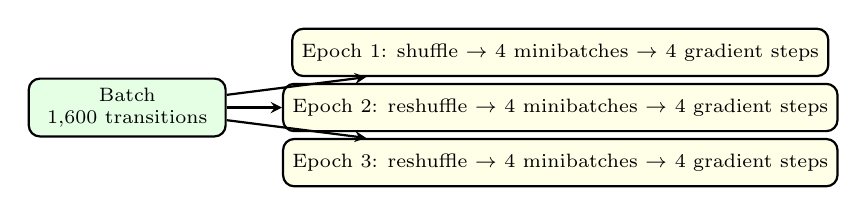
\begin{tikzpicture}[
    box/.style={draw, rounded corners, minimum height=0.6cm, align=center,
                font=\scriptsize, thick, minimum width=2.5cm},
    arrow/.style={->, thick, >=stealth}
  ]
    \node[box, fill=green!10] (batch) at (0,0) {Batch\\1{,}600 transitions};
    \node[box, fill=yellow!10] (e1) at (5.5, 0.7) {Epoch 1: shuffle $\to$ 4 minibatches $\to$ 4 gradient steps};
    \node[box, fill=yellow!10] (e2) at (5.5, 0.0) {Epoch 2: reshuffle $\to$ 4 minibatches $\to$ 4 gradient steps};
    \node[box, fill=yellow!10] (e3) at (5.5,-0.7) {Epoch 3: reshuffle $\to$ 4 minibatches $\to$ 4 gradient steps};
    \draw[arrow] (batch) -- (e1);
    \draw[arrow] (batch) -- (e2);
    \draw[arrow] (batch) -- (e3);
  \end{tikzpicture}
  \end{center}

  \begin{itemize}\setlength\itemsep{1pt}
    \item \textbf{epochs = 1}: see each transition once, compute gradient, discard batch.
    \item \textbf{epochs = 4}: four passes with different minibatch groupings
      $\Rightarrow$ extract $4\times$ more signal from the same data.
    \item \textbf{Safety valve:} \texttt{target\_kl = 0.01} stops early
      if the policy diverges too far from the rollout policy.
  \end{itemize}

  \smallskip
  \textbf{Key insight:} epochs compensate for small batches.
  \begin{center}
  \footnotesize
  \begin{tabular}{lrrr}
    \toprule
    & \textbf{Batch} & \textbf{Epochs} & \textbf{Effective data} \\
    \midrule
    Paper          & 5{,}600 & 1 & 5{,}600 \\
    Ours (ep$=$1)  & 1{,}600 & 1 & 1{,}600 \\
    \rowcolor{highlight}
    Ours (ep$=$4)  & 1{,}600 & 4 & \textbf{6{,}400} \\
    \bottomrule
  \end{tabular}
  \end{center}
\end{frame}

% ──────────────────────────────────────────────────────────────────────────────
\begin{frame}{The Role of Epochs: What ``Four Passes'' Means Concretely}
  \small
  \textbf{Setup:} We have a batch of 1{,}600 transitions (indexed $t_1, t_2, \ldots, t_{1600}$).
  The \textbf{minibatch count} is 4, so each minibatch has $1600 / 4 = 400$ transitions.

  \medskip
  \textbf{One ``pass'' (= one epoch):}
  \begin{enumerate}\setlength\itemsep{1pt}
    \item \textbf{Shuffle} the 1{,}600 transitions into a random permutation
    \item \textbf{Split} the shuffled sequence into 4 consecutive chunks of 400:
      \begin{center}\scriptsize
      \begin{tabular}{llll}
        Minibatch A: & $t_{731}, t_{42}, t_{1588}, \ldots$ & (400 transitions) & $\to$ gradient step 1 \\
        Minibatch B: & $t_{205}, t_{1103}, t_{8}, \ldots$  & (400 transitions) & $\to$ gradient step 2 \\
        Minibatch C: & $t_{1440}, t_{67}, t_{889}, \ldots$ & (400 transitions) & $\to$ gradient step 3 \\
        Minibatch D: & $t_{512}, t_{1299}, t_{33}, \ldots$ & (400 transitions) & $\to$ gradient step 4 \\
      \end{tabular}
      \end{center}
    \item Each minibatch computes a \textbf{separate gradient step}: forward pass $\to$ loss $\to$ backward $\to$ Adam update
  \end{enumerate}

  \medskip
  \textbf{``Four passes'' (epochs = 4):} Repeat the above 4 times, with a
  \emph{fresh random shuffle} each time.  Every transition appears in exactly
  one minibatch per epoch, but in a \emph{different} minibatch each epoch.

  \smallskip
  \begin{center}\scriptsize
  \begin{tabular}{lcccc}
    \toprule
    & \textbf{Epoch 1} & \textbf{Epoch 2} & \textbf{Epoch 3} & \textbf{Epoch 4} \\
    \midrule
    Transition $t_{42}$  & Minibatch A & Minibatch C & Minibatch B & Minibatch D \\
    Transition $t_{205}$ & Minibatch B & Minibatch A & Minibatch D & Minibatch C \\
    \bottomrule
  \end{tabular}
  \end{center}

  \textbf{Total gradient steps per update:} $4 \text{ epochs} \times 4 \text{ minibatches} = 16$ gradient steps,
  using the same 1{,}600 transitions (but in different random groupings each time).
\end{frame}

% ══════════════════════════════════════════════════════════════════════════════
\section{Scaled-Down Subset}
% ══════════════════════════════════════════════════════════════════════════════

% ──────────────────────────────────────────────────────────────────────────────
\begin{frame}{Subset Design: 147 Instances}
  \textbf{Method:} Stratified sampling with \texttt{every\_k=10} from each $(n, |w|)$ cell.

  \medskip
  \begin{columns}[T]
    \begin{column}{0.45\textwidth}
      \small
      \begin{tabular}{crr}
        \toprule
        $|w|$ & \textbf{Full cell} & \textbf{Sampled} \\
        \midrule
        1--3 & 2 each  & 1 each \\
        4    & 6       & 1 \\
        5    & 18      & 2 \\
        6    & 42      & 5 \\
        7    & 98      & 10 \\
        \midrule
        \multicolumn{2}{l}{\textbf{Per $n$-row:}} & \textbf{21} \\
        \multicolumn{2}{l}{\textbf{Total} ($7 \times 21$):} & \textbf{147} \\
        \bottomrule
      \end{tabular}
    \end{column}
    \begin{column}{0.52\textwidth}
      \textbf{Why this works:}
      \begin{itemize}
        \item Every $(n, |w|)$ cell has $\ge 1$ instance\\
          $\Rightarrow$ full difficulty coverage
        \item Easy baseline ($|w| \le 3$, 100\% greedy)\\
          retained for sanity checks
        \item Hard frontier ($|w| = 6{,}7$ at high $n$)\\
          has 5--10 instances for statistical power
        \item Reuses existing code:\\
          \texttt{load\_stratified\_subset(d, every\_k=10)}
      \end{itemize}
    \end{column}
  \end{columns}

  \bigskip
  \footnotesize 12.4\% of full dataset.  Expected greedy baseline: $\sim$46\% (matches full dataset rate).
\end{frame}

% ──────────────────────────────────────────────────────────────────────────────
\begin{frame}{What Do $n$ and $|w|$ Control?}
  \small
  The Miller--Schupp series $\mathrm{MS}(n, w)$ is parameterised by two values:

  \medskip
  \textbf{Parameter $n$: controls the first relator.}
  \[
    r_0 = \inv{x}\, y^n\, x\, y^{-(n+1)}
  \]
  Higher $n$ $\Rightarrow$ longer $r_0$ $\Rightarrow$ larger search space.
  From the paper (Section 3.3, Figure 1): solve rate \textbf{decreases monotonically with $n$}.

  \medskip
  \textbf{Parameter $|w|$: controls the second relator.}
  \[
    r_1 = \inv{x}\, w \quad\text{where } w \text{ has zero exponent sum on } x
  \]
  Higher $|w|$ $\Rightarrow$ more complex $w$ $\Rightarrow$ more ``entangled'' presentation.

  \medskip
  \begin{block}{Key Theoretical Result (Theorem 2, p13)}
    $\mathrm{MS}(1, w)$ is \textbf{AC-trivial for all $w$}.
    This explains why greedy solves 100\% of $n{=}1$ instances --- these are provably easy.
    The paper also notes that greedy solved \emph{all} $n{=}1$ instances in the full dataset.
  \end{block}

  \medskip
  \textbf{Hardness gradient:} difficulty increases with both $n$ and $|w|$, but $n$
  is the stronger driver of hardness (especially $n \ge 4$).
\end{frame}

% ──────────────────────────────────────────────────────────────────────────────
\begin{frame}{The Role of $|w|$: Examples and Paper Observations}
  \small
  \textbf{Concrete examples} (all with $n = 2$, so $r_0 = \inv{x} y^2 x y^{-3}$):
  \begin{center}
  \begin{tabular}{clrl}
    \toprule
    $|w|$ & $w$ & $r_1 = \inv{x}\, w$ & \textbf{Greedy?} \\
    \midrule
    1 & $y$ & $\inv{x}\, y$ & \textcolor{good}{Solved} \\
    3 & $y \inv{x} x$ & $\inv{x}\, y\, \inv{x}\, x$ & \textcolor{good}{Solved} \\
    5 & $y^2 \inv{x} y \inv{y} x$ & $\inv{x}\, y^2\, \inv{x}\, y\, \inv{y}\, x$ & Depends \\
    7 & (98 possibilities) & & Many \textcolor{bad}{unsolved} \\
    \bottomrule
  \end{tabular}
  \end{center}

  \medskip
  \textbf{Paper observation} (Section 3.3, Figure 1b):
  \begin{itemize}\setlength\itemsep{2pt}
    \item Greedy solve rate is \emph{less sensitive} to $|w|$ than to $n$.
    \item At fixed $n$, larger $|w|$ sometimes \emph{helps} --- longer words
      offer more free-reduction opportunities when concatenated.
    \item But the \textbf{hardest unsolved instances} tend to have both high $n$
      \emph{and} high $|w|$ --- the combination creates deeply entangled presentations
      that require long sequences of AC moves to untangle.
    \item For PPO, the dataset is dominated by high-$|w|$ instances:
      82\% have $|w| \ge 6$, so performance on $|w| = 6, 7$ is critical.
  \end{itemize}
\end{frame}

% ──────────────────────────────────────────────────────────────────────────────
\begin{frame}{The Role of $|w|$: Second Relator Complexity}
  \small
  While $n$ controls the first relator, $|w|$ controls the \textbf{combinatorial complexity}
  of the second relator $r_1 = \inv{x}\, w$.

  \medskip
  \textbf{What does $|w|$ encode?}
  \begin{itemize}\setlength\itemsep{2pt}
    \item $w$ is a word in $\{x, \inv{x}, y, \inv{y}\}$ with \textbf{zero exponent sum on $x$}
      (i.e., \#$x$ = \#$\inv{x}$ in $w$).
    \item $|w| = 1$: only $w = y$ or $w = \inv{y}$ (2 choices per $n$).
    \item $|w| = 7$: 98 distinct words after removing cyclic permutations.
    \item Higher $|w|$ $\Rightarrow$ more ways to ``entangle'' the generators
      $\Rightarrow$ more complex interaction between $r_0$ and $r_1$.
  \end{itemize}

\end{frame}

% ──────────────────────────────────────────────────────────────────────────────
\begin{frame}{Full Dataset Distribution (Reference)}
  Each $(n, |w|)$ cell has identical counts across all $n$ values:

  \medskip
  \begin{center}
  \small
  \begin{tabular}{c|ccccccc|r}
    \toprule
    $n \backslash |w|$ & 1 & 2 & 3 & 4 & 5 & 6 & 7 & \textbf{Total} \\
    \midrule
    1 & 2 & 2 & 2 & 6 & 18 & 42 & 98 & 170 \\
    2 & 2 & 2 & 2 & 6 & 18 & 42 & 98 & 170 \\
    3 & 2 & 2 & 2 & 6 & 18 & 42 & 98 & 170 \\
    4 & 2 & 2 & 2 & 6 & 18 & 42 & 98 & 170 \\
    5 & 2 & 2 & 2 & 6 & 18 & 42 & 98 & 170 \\
    6 & 2 & 2 & 2 & 6 & 18 & 42 & 98 & 170 \\
    7 & 2 & 2 & 2 & 6 & 18 & 42 & 98 & 170 \\
    \midrule
    \textbf{Total} & 14 & 14 & 14 & 42 & 126 & 294 & 686 & \textbf{1190} \\
    \bottomrule
  \end{tabular}
  \end{center}

  \bigskip
  \begin{itemize}
    \item $n$ controls first relator complexity ($r_0 = \inv{x}\, y^n\, x\, y^{-(n+1)}$)
    \item $|w|$ controls second relator length ($r_1 = \inv{x}\, w$)
    \item 82\% of instances have $|w| \ge 6$ --- the dataset is dominated by hard cases
  \end{itemize}
\end{frame}

% ══════════════════════════════════════════════════════════════════════════════
\section{Classical Baselines on Subset}
% ══════════════════════════════════════════════════════════════════════════════

% ──────────────────────────────────────────────────────────────────────────────
\begin{frame}[fragile]{Classical Baselines: Subset vs.\ Full Dataset}
  \begin{center}
  \begin{tabular}{lrrrr}
    \toprule
    \textbf{Algorithm} & \textbf{Subset} & \textbf{Subset \%} & \textbf{Full \%} & \textbf{Match?} \\
    \midrule
    Greedy ($10^6$ nodes) & \textbf{71} / 147 & \textbf{48.3\%} & 46.6\% & \textcolor{good}{\checkmark} \\
    BFS ($10^6$ nodes)    & 42 / 147           & 28.6\%           & 23.4\% & \textcolor{good}{$\approx$} \\
    \bottomrule
  \end{tabular}
  \end{center}

  \bigskip
  \textbf{Subset is representative:} solve rates match full dataset within $\sim$2--5 percentage points.

  \bigskip
  BFS slightly higher on subset (28.6\% vs.\ 23.4\%) because stratified sampling
  overrepresents small cells ($|w| \le 3$) where both algorithms solve 100\%.

  \bigskip
  \textbf{Commands:}
  \begin{lstlisting}[language=bash]
python -m ac_solver.search.miller_schupp.evaluate \
    --search-fn greedy --max-nodes 1000000 --workers 4 --every-k 10
python -m ac_solver.search.miller_schupp.evaluate \
    --search-fn bfs --max-nodes 1000000 --workers 2 --every-k 10
  \end{lstlisting}
\end{frame}

% ──────────────────────────────────────────────────────────────────────────────
\begin{frame}{Greedy Baseline: Per-$(n, |w|)$ Solve Rates on Subset}
  \footnotesize
  \begin{center}
  \begin{tabular}{c|ccccccc|r}
    \toprule
    $n \backslash |w|$ & 1 & 2 & 3 & 4 & 5 & 6 & 7 & \textbf{Row} \\
    \midrule
    1 & \cellcolor{good!30}1/1 & \cellcolor{good!30}1/1 & \cellcolor{good!30}1/1 & \cellcolor{good!30}1/1 & \cellcolor{good!30}2/2 & \cellcolor{good!30}5/5 & \cellcolor{good!30}10/10 & \textcolor{good}{\textbf{21/21}} \\
    2 & \cellcolor{good!30}1/1 & \cellcolor{good!30}1/1 & \cellcolor{good!30}1/1 & \cellcolor{good!30}1/1 & \cellcolor{good!30}2/2 & \cellcolor{good!15}4/5 & \cellcolor{neutral!20}6/10 & 16/21 \\
    3 & \cellcolor{good!30}1/1 & \cellcolor{good!30}1/1 & \cellcolor{good!30}1/1 & \cellcolor{bad!20}0/1 & \cellcolor{bad!15}1/2 & \cellcolor{good!15}4/5 & \cellcolor{bad!20}3/10 & 11/21 \\
    4 & \cellcolor{good!30}1/1 & \cellcolor{good!30}1/1 & \cellcolor{good!30}1/1 & \cellcolor{bad!20}0/1 & \cellcolor{bad!30}0/2 & \cellcolor{bad!20}1/5 & \cellcolor{bad!20}2/10 & 6/21 \\
    5 & \cellcolor{good!30}1/1 & \cellcolor{good!30}1/1 & \cellcolor{good!30}1/1 & \cellcolor{bad!20}0/1 & \cellcolor{bad!30}0/2 & \cellcolor{bad!15}2/5 & \cellcolor{bad!15}4/10 & 9/21 \\
    6 & \cellcolor{good!30}1/1 & \cellcolor{good!30}1/1 & \cellcolor{good!30}1/1 & \cellcolor{bad!20}0/1 & \cellcolor{bad!30}0/2 & \cellcolor{bad!20}1/5 & \cellcolor{bad!30}0/10 & 4/21 \\
    7 & \cellcolor{good!30}1/1 & \cellcolor{good!30}1/1 & \cellcolor{good!30}1/1 & \cellcolor{bad!20}0/1 & \cellcolor{bad!30}0/2 & \cellcolor{bad!20}1/5 & \cellcolor{bad!30}0/10 & 4/21 \\
    \bottomrule
  \end{tabular}
  \end{center}

  \bigskip
  \begin{itemize}
    \item \textbf{$|w| \le 3$:} 100\% solved (all cells have size 1, all trivially easy)
    \item \textbf{$n = 1$:} 100\% solved regardless of $|w|$ (MS(1,$w$) is AC-trivial for all $w$)
    \item \textbf{Hard frontier} ($n \ge 4$, $|w| \ge 4$): steep drop-off, 0--40\% solve rate
    \item PPO must beat this baseline to demonstrate value
  \end{itemize}
\end{frame}

% ──────────────────────────────────────────────────────────────────────────────
\begin{frame}{BFS Baseline: Per-$(n, |w|)$ Solve Rates on Subset}
  \footnotesize
  \begin{center}
  \begin{tabular}{c|ccccccc|r}
    \toprule
    $n \backslash |w|$ & 1 & 2 & 3 & 4 & 5 & 6 & 7 & \textbf{Row} \\
    \midrule
    1 & \cellcolor{good!30}1/1 & \cellcolor{good!30}1/1 & \cellcolor{good!30}1/1 & \cellcolor{good!30}1/1 & \cellcolor{good!30}2/2 & \cellcolor{bad!15}2/5 & \cellcolor{bad!15}5/10 & 13/21 \\
    2 & \cellcolor{good!30}1/1 & \cellcolor{good!30}1/1 & \cellcolor{good!30}1/1 & \cellcolor{bad!20}0/1 & \cellcolor{bad!30}0/2 & \cellcolor{bad!15}3/5 & \cellcolor{bad!15}4/10 & 10/21 \\
    3 & \cellcolor{good!30}1/1 & \cellcolor{good!30}1/1 & \cellcolor{good!30}1/1 & \cellcolor{bad!20}0/1 & \cellcolor{bad!30}0/2 & \cellcolor{bad!20}1/5 & \cellcolor{bad!30}0/10 & 4/21 \\
    4 & \cellcolor{good!30}1/1 & \cellcolor{good!30}1/1 & \cellcolor{good!30}1/1 & \cellcolor{bad!20}0/1 & \cellcolor{bad!30}0/2 & \cellcolor{bad!20}1/5 & \cellcolor{bad!30}0/10 & 4/21 \\
    5 & \cellcolor{good!30}1/1 & \cellcolor{good!30}1/1 & \cellcolor{good!30}1/1 & \cellcolor{bad!20}0/1 & \cellcolor{bad!30}0/2 & \cellcolor{bad!20}1/5 & \cellcolor{bad!30}0/10 & 4/21 \\
    6 & \cellcolor{good!30}1/1 & \cellcolor{good!30}1/1 & \cellcolor{good!30}1/1 & \cellcolor{bad!20}0/1 & \cellcolor{bad!30}0/2 & \cellcolor{bad!20}1/5 & \cellcolor{bad!30}0/10 & 4/21 \\
    7 & \cellcolor{good!30}1/1 & \cellcolor{good!30}1/1 & \cellcolor{good!30}1/1 & \cellcolor{bad!20}0/1 & \cellcolor{bad!30}0/2 & \cellcolor{bad!30}0/5 & \cellcolor{bad!30}0/10 & 3/21 \\
    \bottomrule
  \end{tabular}
  \end{center}

  \bigskip
  \begin{itemize}
    \item BFS drops off faster than greedy: 42/147 vs.\ 71/147
    \item BFS guarantees \textbf{shortest paths} but exhausts $10^6$-node budget sooner
    \item For $n \ge 3$: BFS solves only $|w| \le 3$ cells (with rare exceptions)
    \item \textbf{Gap:} greedy solves 29 instances that BFS cannot within budget
  \end{itemize}
\end{frame}

% ══════════════════════════════════════════════════════════════════════════════
\section{PPO Ablation Design}
% ══════════════════════════════════════════════════════════════════════════════

% ──────────────────────────────────────────────────────────────────────────────
\begin{frame}{Ablation Design: 3 Runs, 2 Factors}
  \textbf{Sequential ablation design:} isolate each factor one at a time.

  \medskip
  \begin{center}
  \small
  \begin{tabular}{clcclp{4.5cm}}
    \toprule
    \textbf{Run} & \textbf{Label} & \textbf{Reward fix} & \textbf{Epochs} & \textbf{Purpose} \\
    \midrule
    0 & \texttt{diag\_baseline}      & No  & 1 & Control (broken config) \\
    1 & \texttt{diag\_reward\_fix}   & \textcolor{good}{Yes} & 1 & Isolate reward fix \\
    2 & \texttt{diag\_reward\_epochs}& \textcolor{good}{Yes} & \textcolor{good}{4} & Reward fix $+$ data reuse \\
    \bottomrule
  \end{tabular}
  \end{center}

  \bigskip
  \begin{itemize}
    \item \textbf{Factor 1: Reward scaling} (\texttt{--skip-reward-division}).
      Removes \texttt{rewards /= 14400} so PPO sees $[-10, +1000]$ matching the paper.
    \item \textbf{Factor 2: \texttt{update\_epochs}} ($1 \to 4$).
      Paper uses 1 with batch${}=5{,}600$; we have batch${}=1{,}600$.
      With epochs${}=4$, effective data $= 6{,}400 >$ paper's $5{,}600$.
    \item \textbf{Budget:} 3 $\times$ 10M steps $=$ 30M total.
    \item \textbf{Single seed} ($s{=}1$): looking for large effects, not small statistical differences.
  \end{itemize}
\end{frame}

% ──────────────────────────────────────────────────────────────────────────────
\begin{frame}{Fixed Hyperparameters (Same Across All Runs)}
  \footnotesize
  \begin{center}
  \begin{tabular}{lrll}
    \toprule
    \textbf{Parameter} & \textbf{Value} & \textbf{Source} & \textbf{Rationale} \\
    \midrule
    \texttt{num\_envs}    & 8       & Hardware     & Mac limit; held constant \\
    \texttt{num\_steps}   & 200     & Paper \S4.4  & Constant-horizon setup \\
    \texttt{batch\_size}  & 1{,}600 & $8 \times 200$ & Constrained by above \\
    \texttt{nodes}        & $[512, 512]$ & Paper App.\ A & 2-layer MLP \\
    $\gamma$              & 0.999   & Paper App.\ A & Effective horizon $\sim$1000 \\
    $\lambda_\text{GAE}$  & 0.95    & Paper App.\ A & Bias-variance trade-off \\
    $\epsilon_\text{clip}$& 0.2     & Paper App.\ A & PPO clipping \\
    $c_\text{ent}$        & 0.01    & Paper App.\ A & Exploration bonus \\
    $c_\text{vf}$         & 0.5     & Paper App.\ A & Value loss coefficient \\
    \texttt{target\_kl}   & 0.01    & Paper App.\ A & Early stop in epoch loop \\
    \texttt{max\_grad\_norm}& 0.5   & Paper App.\ A & Gradient clipping \\
    Adam $\epsilon$       & $10^{-5}$& Paper App.\ A & Numerical stability \\
    \texttt{repeat\_solved\_prob} & 0.25 & Paper \S4.4 & Curriculum \\
    \texttt{seed}         & 1       & Convention   & Fixed for reproducibility \\
    LR schedule           & linear$\to$0 & Paper App.\ A & Same across all 3 runs \\
    \bottomrule
  \end{tabular}
  \end{center}
\end{frame}

% ──────────────────────────────────────────────────────────────────────────────
\begin{frame}{Varied Factors: Justification}
  \small
  \textbf{Factor 1: Reward scaling} (\texttt{--skip-reward-division})
  \begin{itemize}
    \item Removes \texttt{rewards /= 14400} from \texttt{training.py}
    \item PPO sees $[-10, +1000]$ matching the paper exactly
    \item Expected to help the critic learn meaningful value differences
  \end{itemize}

  \medskip
  \textbf{Factor 2: \texttt{update\_epochs}} ($1 \to 4$)
  \begin{itemize}
    \item Paper uses 1; standard PPO uses 3--10
    \item At batch size 1{,}600 (small), single-pass extracts minimal signal
    \item With epochs${}=4$: effective data $= 1{,}600 \times 4 = 6{,}400$,
      exceeding the paper's $5{,}600$ per update
    \item \texttt{target\_kl=0.01} prevents overfitting per epoch
  \end{itemize}

  \medskip
  \begin{block}{Why Not LR Schedule?}
    We did not run cosine LR experiments (originally planned as Runs 3 and 4).
    At 10M steps, linear and cosine schedules are nearly identical ---
    this factor only matters for long runs ($>$50M).
    We prioritised the two factors most likely to matter at this training budget.
  \end{block}
\end{frame}

% ──────────────────────────────────────────────────────────────────────────────
\begin{frame}{Success Criteria (Before Looking at Results)}
  \begin{center}
  \begin{tabular}{lll}
    \toprule
    \textbf{Criterion} & \textbf{Threshold} & \textbf{Interpretation} \\
    \midrule
    Reward fix works        & Run 1 $> 2\times$ Run 0 & Division was the cause \\
    Epochs help             & Run 2 $>$ Run 1 by $>$30\% & Data reuse matters \\
    Combined viable         & Run 2 $>$ 5/147 (3.4\%) & Worth extending to 50M \\
    Approaching paper       & Run 2 $>$ 15/147 (10\%) & Could match paper at scale \\
    \midrule
    Baselines hold          & Greedy $\approx$ 46\% & Subset is representative \\
    \bottomrule
  \end{tabular}
  \end{center}

  \bigskip
  \textcolor{good}{\checkmark} \textbf{Baselines confirmed:} Greedy 48.3\%, BFS 28.6\%
\end{frame}

% ══════════════════════════════════════════════════════════════════════════════
\section{Why Epochs = 4 is the Critical Fix}
% ══════════════════════════════════════════════════════════════════════════════

% ──────────────────────────────────────────────────────────────────────────────
\begin{frame}{Key Insight: \texttt{norm\_adv} Makes Reward Scale Less Important}
  \small
  Recall that the PPO policy gradient uses \emph{normalised} advantages (\texttt{norm\_adv=True}):
  \[
    \hat{A}_t^\text{norm} = \frac{\hat{A}_t - \bar{A}}{\sigma_A + 10^{-8}}
    \qquad\Longrightarrow\qquad
    \text{mean} \approx 0,\; \text{std} \approx 1 \;\;\textbf{regardless of reward scale}
  \]

  \medskip
  \begin{center}
  \footnotesize
  \begin{tabular}{lrrrr}
    \toprule
    & \multicolumn{2}{c}{\textbf{Before norm}} & \multicolumn{2}{c}{\textbf{After norm}} \\
    \cmidrule(lr){2-3} \cmidrule(lr){4-5}
    & $\bar{A}$ & $\sigma_A$ & $\bar{A}^\text{norm}$ & $\sigma_A^\text{norm}$ \\
    \midrule
    Run 0 ($\div 14400$) & $-0.001$ & $0.11$ & $\approx 0$ & $\approx 1$ \\
    Run 1 (no $\div$)    & $-174$   & $37$   & $\approx 0$ & $\approx 1$ \\
    \bottomrule
  \end{tabular}
  \end{center}

  \medskip
  \alert{The actor receives \emph{identical} gradient magnitudes in both runs.}

  \bigskip
  \begin{block}{Implication}
    The reward fix helps the \emph{critic} learn real value differences, but the
    \emph{policy} is insensitive to reward scale because normalisation removes it.
    The dominant bottleneck was \textbf{data reuse} (\texttt{epochs}), not reward scale.
    This explains why Run~1 (reward fix only) $\approx$ Run~0 in evaluation.
  \end{block}
\end{frame}

% ──────────────────────────────────────────────────────────────────────────────
\begin{frame}{Why \texttt{epochs=4} is the Critical Fix}
  \small
  \textbf{Mathematical analysis:} The signal-to-noise ratio (SNR) of the policy gradient
  scales with the effective number of samples:
  \[
    \text{SNR}_\text{policy} \;\propto\; \frac{\sqrt{N_\text{eff}}}{\sigma_A}
    \quad\text{where}\quad
    N_\text{eff} \approx \text{batch} \times \text{epochs}
  \]

  \begin{center}
  \begin{tabular}{lrrrr}
    \toprule
    \textbf{Configuration} & \textbf{Batch} & \textbf{Epochs} & $N_\text{eff}$ & \textbf{Relative SNR} \\
    \midrule
    Paper (28 envs)  & 5{,}600 & 1 & 5{,}600 & $1.00\times$ \\
    Run 0/1 (8 envs) & 1{,}600 & 1 & 1{,}600 & $0.53\times$ \\
    \rowcolor{highlight}
    \textbf{Run 2} (8 envs, ep=4) & 1{,}600 & \textbf{4} & \textbf{6{,}400} & $\mathbf{1.07\times}$ \\
    \bottomrule
  \end{tabular}
  \end{center}

  \medskip
  \textbf{Key point:} With epochs${}=1$, our gradient SNR is only 53\% of the paper's.
  The policy gradient is too noisy to learn --- effectively a random walk in parameter space.

  \medskip
  With epochs${}=4$, SNR \emph{exceeds} the paper's setup.  This is the cheapest possible
  fix: zero additional environment steps, only extra gradient computation.
\end{frame}

% ──────────────────────────────────────────────────────────────────────────────
\begin{frame}{How $\sigma_A$ Is Computed: Advantage Normalisation in Detail}
  \small
  The advantage standard deviation $\sigma_A$ in the SNR formula comes from
  \texttt{norm\_adv} (line 404 of \texttt{training.py}):
  \[
    \hat{A}_t^\text{norm} = \frac{\hat{A}_t - \bar{A}}{\sigma_A + 10^{-8}}
    \quad\text{where}\quad
    \bar{A} = \frac{1}{M}\sum_{i=1}^M \hat{A}_i, \;\;
    \sigma_A = \sqrt{\frac{1}{M}\sum_{i=1}^M (\hat{A}_i - \bar{A})^2}
  \]
  Here $M = 400$ (minibatch size). The statistics are computed \textbf{per minibatch},
  not over the full batch.
\end{frame}

% ──────────────────────────────────────────────────────────────────────────────
\begin{frame}{Advantage Normalisation: Worked Example and Implications}
  \footnotesize
  \textbf{Worked example} (one minibatch of 400 transitions at 10M):
  \begin{center}
  \begin{tabular}{lrrl}
    \toprule
    & \textbf{Run 0} ($\div 14400$) & \textbf{Run 1} (paper scale) & \\
    \midrule
    Raw advantages $\hat{A}_i$ & $[-0.15, +0.12]$ & $[-250, +180]$ & Range \\
    $\bar{A}$ & $-0.001$ & $-160$ & Mean \\
    $\sigma_A$ & $0.063$ & $36.2$ & Std dev \\
    \midrule
    After norm: $\bar{A}^\text{norm}$ & $\approx 0$ & $\approx 0$ & \textbf{Same} \\
    After norm: $\sigma_A^\text{norm}$ & $\approx 1$ & $\approx 1$ & \textbf{Same} \\
    \bottomrule
  \end{tabular}
  \end{center}

  \medskip
  \textbf{Normalisation removes scale differences.  What it cannot fix:}
  \begin{itemize}\setlength\itemsep{2pt}
    \item If all raw advantages are nearly identical (critic gives constant $V$),
      normalisation \textbf{amplifies noise into signal} $\Rightarrow$ random gradient directions.
    \item The $\sigma_A$ denominator \emph{scales up} tiny fluctuations into unit variance ---
      a minibatch where $\hat{A}_i \in [-0.002, +0.001]$ becomes $\hat{A}_i^\text{norm} \in [-1.3, +0.7]$.
    \item More epochs help: averaging over 16 reshuffled minibatch gradients (instead of 4)
      cancels out the noise that normalisation amplified.
  \end{itemize}

  \medskip
  \textbf{Bottom line:} \texttt{norm\_adv} is scale-invariant but \textbf{not noise-invariant}.
  A better critic (from reward fix) gives more \emph{structured} advantages.
  More epochs extract that structure despite per-minibatch noise.
\end{frame}

% ──────────────────────────────────────────────────────────────────────────────
\begin{frame}{The Epoch Mechanism: Multiple Gradient Steps}
  \small
  Each epoch \textbf{reshuffles} the batch into new minibatches, creating diverse
  gradient estimates from the same data:

  \medskip
  \begin{center}
  \footnotesize
  \begin{tabular}{lp{9cm}}
    \toprule
    \textbf{Epoch} & \textbf{Minibatch composition} \\
    \midrule
    1 & Shuffle 1{,}600 transitions $\to$ 4 minibatches of 400 $\to$ 4 gradient steps \\
    2 & \textbf{Reshuffle} $\to$ different groupings of 400 $\to$ 4 new gradient steps \\
    3 & Reshuffle $\to$ yet different groupings $\to$ 4 more gradient steps \\
    4 & Reshuffle $\to$ final groupings $\to$ 4 final gradient steps \\
    \midrule
    \textbf{Total} & \textbf{16 gradient steps} per PPO update (vs.\ 4 with epochs${}=1$) \\
    \bottomrule
  \end{tabular}
  \end{center}

  \medskip
  \textbf{Why reshuffling matters:}
  \begin{itemize}\setlength\itemsep{1pt}
    \item Each minibatch of 400 sees a \emph{different random subset} of the 1{,}600 transitions
    \item Different subsets produce different gradient directions
    \item Averaging over 16 steps (instead of 4) reduces gradient variance by $\sim 2\times$
    \item This is analogous to training a neural network for multiple epochs on a fixed dataset
  \end{itemize}

  \medskip
  The net effect: each PPO update extracts $4\times$ more information from the same
  rollout data, at the cost of $4\times$ more gradient computation (cheap on GPU).
\end{frame}

% ──────────────────────────────────────────────────────────────────────────────
\begin{frame}{Epochs vs.\ Batch Size: A Mathematical Equivalence}
  \small
  \textbf{Claim:} $K$ epochs with batch $B$ $\approx$ batch $B \cdot K$ in terms of gradient variance.

  \medskip
  With i.i.d.\ samples, gradient variance scales as:
  \[
    \mathrm{Var}[\nabla \mathcal{L}] \;\propto\; \frac{\sigma^2}{N}
  \]

  \begin{center}
  \begin{tabular}{lrrrl}
    \toprule
    & \textbf{Batch} & \textbf{Epochs} & \textbf{Grad steps} & \textbf{Variance} \\
    \midrule
    Batch $= B \cdot K$, ep${}=1$ & $BK$ & 1 & $BK / M$ & $\sigma^2 / BK$ \\
    Batch $= B$, ep${}=K$ & $B$ & $K$ & $K \cdot B / M$ & $\approx \sigma^2 / BK$ \\
    \bottomrule
  \end{tabular}
  \end{center}

  \medskip
  \textbf{Caveat --- staleness:}
  \begin{itemize}\setlength\itemsep{1pt}
    \item With a larger batch, all samples are fresh (collected under current policy $\pi_{\theta_\text{old}}$)
    \item With multiple epochs, later epochs use slightly \emph{stale} data:
      the policy has already moved from $\pi_{\theta_\text{old}}$
    \item PPO's clipping mechanism limits this drift (next slide)
    \item In practice, epochs${}=4$ with \texttt{target\_kl=0.01} works well because
      the policy moves very little per update
  \end{itemize}
\end{frame}

% ──────────────────────────────────────────────────────────────────────────────
\begin{frame}{PPO Clipping Prevents Epoch Overfitting}
  \small
  \textbf{How PPO stays safe with multiple epochs:}

  \medskip
  The probability ratio $r_t(\theta) = \pi_\theta(a_t \mid s_t) / \pi_{\theta_\text{old}}(a_t \mid s_t)$
  is \textbf{clipped} to $[1 - \epsilon,\; 1 + \epsilon]$ with $\epsilon = 0.2$:
  \[
    L^{CLIP} = \min\!\big( r_t A_t,\;\; \mathrm{clip}(r_t, 0.8, 1.2)\, A_t \big)
  \]

  Once $r_t$ hits the clip boundary, further gradient steps on that transition
  produce \textbf{zero gradient} --- the clipping acts as a per-sample learning rate schedule.

  \medskip
  \textbf{Additional safety: \texttt{target\_kl = 0.01}}

  After each epoch, we compute the approximate KL divergence:
  \[
    D_\text{KL}(\pi_{\theta_\text{old}} \| \pi_\theta) \approx
    \mathbb{E}_t\!\left[\frac{(r_t - 1)^2}{2}\right]
  \]
  If $D_\text{KL} > 0.01$, the epoch loop \textbf{terminates early},
  discarding remaining epochs for this update.

  \medskip
  \textbf{Result:} At 700K steps, Run 2 shows clipfrac $= 0.0016$ and
  approx\_kl $= 0.0013$ --- the policy moves gently even with 4 epochs.
  Most transitions are not clipped; the policy is safely extracting signal.
\end{frame}

% ──────────────────────────────────────────────────────────────────────────────
\begin{frame}{Empirical Evidence: Epochs Change Everything}
  \small
  Training metrics comparison at $\sim$700K steps:

  \begin{center}
  \footnotesize
  \begin{tabular}{lrrrl}
    \toprule
    \textbf{Metric} & \textbf{Run 0} & \textbf{Run 1} & \textbf{Run 2} & \textbf{Interpretation} \\
    \midrule
    entropy     & 2.484 & 2.483 & \textcolor{good}{\textbf{2.065}} & Policy specialising \\
    expl.\ var  & \textcolor{bad}{$-1.42$} & $-0.009$ & \textcolor{good}{$-0.000$} & Critic learning \\
    top-1 prob  & 9.0\% & 9.2\% & \textcolor{good}{\textbf{31.0\%}} & Confident actions \\
    clipfrac    & 0.000 & 0.000 & 0.0016 & Active clipping \\
    approx\_kl  & 0.000 & 0.000 & 0.0013 & Policy updating \\
    policy\_loss& $+0.00005$ & $+0.00004$ & \textcolor{good}{$-0.0148$} & Meaningful gradient \\
    noop rate   & 60.3\% & 59.4\% & 71.1\% & Learned to avoid bad moves \\
    \bottomrule
  \end{tabular}
  \end{center}

  \bigskip
  \textbf{The contrast is dramatic:}
  \begin{itemize}
    \item Runs 0 and 1 (epochs${}=1$): entropy $\approx 2.48$ (near-uniform over 12 actions),
      top-1 $\approx 9\%$, zero clipping. \alert{No learning is happening.}
    \item Run 2 (epochs${}=4$): entropy dropped to 2.06, top-1 jumped to 31\%,
      clipping is active. \textcolor{good}{The policy is differentiating actions.}
  \end{itemize}
\end{frame}

% ══════════════════════════════════════════════════════════════════════════════
\section{PPO Training Results: All Three Runs}
% ══════════════════════════════════════════════════════════════════════════════

% ──────────────────────────────────────────────────────────────────────────────
\begin{frame}{Training Metrics: Run 0 vs.\ Run 1 vs.\ Run 2 at 700K}
  \footnotesize
  \begin{center}
  \begin{tabular}{lrrrl}
    \toprule
    \textbf{Metric} & \textbf{Run 0} & \textbf{Run 1} & \textbf{Run 2} & \textbf{Key difference} \\
    \midrule
    entropy     & 2.484 & 2.483 & \textcolor{good}{2.065} & Run 2: $-0.42$ (policy specialising) \\
    expl.\ var  & $-1.42$ & $-0.009$ & $-0.000$ & Run 1 fixed critic; Run 2 same \\
    top-1 prob  & 9.0\% & 9.2\% & \textcolor{good}{31.0\%} & Run 2: $3.4\times$ more confident \\
    clipfrac    & 0.000 & 0.000 & 0.0016 & Only Run 2 has active clipping \\
    approx\_kl  & 0.000 & 0.000 & 0.0013 & Only Run 2 updates policy \\
    policy\_loss& $+0.00005$ & $+0.00004$ & $-0.0148$ & Run 2: $300\times$ larger magnitude \\
    noop rate   & 60.3\% & 59.4\% & 71.1\% & Run 2 avoids length-increasing moves \\
    \bottomrule
  \end{tabular}
  \end{center}

  \bigskip
  \textbf{Interpretation:}
  \begin{itemize}
    \item \textbf{Run 0 vs.\ Run 1:} The reward fix improved the critic (expl.\ var: $-1.42 \to -0.009$)
      but the \emph{policy} is unchanged (entropy, top-1, clipfrac all identical).
    \item \textbf{Run 1 vs.\ Run 2:} Adding epochs${}=4$ \emph{transforms} the policy.
      The same reward signal, processed $4\times$ more thoroughly, produces genuine learning.
    \item \textbf{Conclusion:} The reward fix was necessary (critic needs real signal)
      but epochs were the \emph{sufficient} condition for policy improvement.
  \end{itemize}
\end{frame}

% ──────────────────────────────────────────────────────────────────────────────
\begin{frame}{Training Metrics at 10M Steps}
  \footnotesize
  \begin{center}
  \begin{tabular}{lrrrl}
    \toprule
    \textbf{Metric} & \textbf{Run 0} & \textbf{Run 1} & \textbf{Run 2} & \textbf{Key difference} \\
    \midrule
    entropy     & 2.449 & 2.467 & \textcolor{good}{\textbf{1.308}} & Run 2: sharp specialisation \\
    expl.\ var  & $-1.75$ & $-0.000$ & \textcolor{good}{$+0.005$} & Run 2 critic slightly positive \\
    top-1 prob  & 12.9\% & 11.7\% & \textcolor{good}{\textbf{52.8\%}} & Run 2: majority action $>$50\% \\
    clipfrac    & 0.000 & 0.000 & 0.000 & Run 2 clipping done (converged) \\
    noop rate   & 61.3\% & 61.8\% & \textcolor{good}{50.6\%} & Run 2 \emph{reduced} noops \\
    \bottomrule
  \end{tabular}
  \end{center}

  \bigskip
  \textbf{Run 2 at 10M vs.\ 700K:}
  \begin{itemize}
    \item Entropy: $2.065 \to 1.308$ --- policy became much more decisive
    \item Top-1: $31\% \to 52.8\%$ --- dominant action selected majority of the time
    \item Noop rate: $71.1\% \to 50.6\%$ --- initially conservative, now taking more risks
    \item Clipfrac: $0.0016 \to 0.000$ --- policy updates have stabilised
  \end{itemize}

  \medskip
  Runs 0 and 1 show \alert{no meaningful change} from 700K to 10M ---
  still near-uniform policies with zero clipping.
\end{frame}

% ──────────────────────────────────────────────────────────────────────────────
\begin{frame}{Why the Reward Fix Didn't Help the \emph{Policy}}
  \small
  The PPO loss function has three terms:
  \[
    \mathcal{L} \;=\; \underbrace{\mathcal{L}_\text{policy}}_{\text{actor gradient}}
    \;-\; c_\text{ent} \cdot H[\pi]
    \;+\; c_\text{vf} \cdot \underbrace{\mathcal{L}_\text{value}}_{\text{critic gradient}}
  \]

  The \textbf{policy gradient} uses \emph{normalised} advantages (\texttt{norm\_adv=True}):
  \[
    \hat{A}_t^\text{norm} = \frac{\hat{A}_t - \bar{A}}{\sigma_A + 10^{-8}}
    \qquad\Longrightarrow\qquad
    \text{mean} \approx 0,\; \text{std} \approx 1 \;\;\textbf{regardless of reward scale}
  \]

  \medskip
  \alert{The actor receives \emph{identical} gradient magnitudes in both Runs 0 and 1.}\\
  Advantage normalisation makes the policy update \textbf{scale-invariant} in the reward.\\
  The reward fix \emph{cannot} improve the actor through this mechanism.

  \medskip
  \begin{block}{Where Does Reward Scale Actually Matter?}
    Reward scale $\to$ critic signal quality $\to$ advantage \emph{direction} (not scale)
    $\to$ policy gradient usefulness.  \texttt{norm\_adv} removes scale; it cannot remove noise.\\
    \textbf{A noisy advantage, once normalised, is still noisy.}
  \end{block}
\end{frame}

% ──────────────────────────────────────────────────────────────────────────────
\begin{frame}{Where Does Reward Scale Actually Matter?}
  \small
  Actor and critic have \textbf{separate parameters} (paper footnote~11 confirms this).
  Adam maintains per-parameter adaptive LR $\Rightarrow$ actor and critic gradients
  \textbf{do not interfere}, even with a single optimiser.

  \medskip
  Reward scale matters for the \textbf{critic's learning quality}, not the actor's gradient magnitude:

  \medskip
  \begin{center}
  \footnotesize
  \begin{tabular}{lp{4.5cm}p{4.5cm}}
    \toprule
    & \textbf{$\div 14{,}400$ (our code)} & \textbf{Paper scale} \\
    \midrule
    Returns & $G_t \in [-0.14, +0.07]$ & $G_t \in [-2000, +1000]$ \\
    Critic target spread & $\sim 0.2$ (all states look the same) & $\sim 3000$ (huge differences) \\
    Critic learning & ``Predict $\approx 0.04$'' fits everything $\Rightarrow$ expl.\ var $+0.66$ but \alert{no per-state signal} & Must learn genuine $V(s)$ differences \\
    Advantage quality & Noise (critic gives constant baseline) & Meaningful signal \\
    \bottomrule
  \end{tabular}
  \end{center}

  \medskip
  \begin{block}{The Real Mechanism}
    Reward scale $\to$ critic signal quality $\to$ advantage \emph{direction} (not scale)
    $\to$ policy gradient usefulness.  \texttt{norm\_adv} removes scale; it cannot remove noise.\\
    \textbf{A noisy advantage, once normalised, is still noisy.}
  \end{block}
\end{frame}

% ══════════════════════════════════════════════════════════════════════════════
\section{PPO Evaluation Results}
% ══════════════════════════════════════════════════════════════════════════════

% ──────────────────────────────────────────────────────────────────────────────
\begin{frame}{Evaluation Results: The Full Picture}
  \small
  \begin{center}
  \begin{tabular}{llrr}
    \toprule
    \textbf{Algorithm} & \textbf{Mode} & \textbf{Solved} & \textbf{Rate} \\
    \midrule
    Greedy ($10^6$ nodes) & --- & \textbf{71}/147 & \textcolor{good}{\textbf{48.3\%}} \\
    BFS ($10^6$ nodes)    & --- & 42/147           & 28.6\% \\
    \midrule
    Run 0 (baseline) 1M   & det / sto$\times$5 & 0 / 1  & 0.0\% / 0.7\% \\
    Run 0 (baseline) 5M   & det / sto$\times$5 & 0 / 1  & 0.0\% / 0.7\% \\
    Run 0 (baseline) 10M  & det / sto$\times$5 & 0 / 2  & 0.0\% / 1.4\% \\
    \midrule
    Run 1 (reward fix) 1M  & det / sto$\times$5 & 0 / 1  & 0.0\% / 0.7\% \\
    Run 1 (reward fix) 5M  & det / sto$\times$5 & 0 / 1  & 0.0\% / 0.7\% \\
    Run 1 (reward fix) 10M & det / sto$\times$5 & 0 / 1  & 0.0\% / 0.7\% \\
    \midrule
    Run 2 (rwd+ep4) 1M     & det / sto$\times$5 & 0 / 2  & 0.0\% / 1.4\% \\
    Run 2 (rwd+ep4) 5M     & det / sto$\times$5 & 0 / 4  & 0.0\% / 2.7\% \\
    \rowcolor{highlight}
    Run 2 (rwd+ep4) 10M    & det / sto$\times$5 & \textcolor{good}{\textbf{8}} / \textcolor{good}{\textbf{10}} & \textcolor{good}{\textbf{5.4\%}} / \textcolor{good}{\textbf{6.8\%}} \\
    \bottomrule
  \end{tabular}
  \end{center}

  \medskip
  \begin{center}
    \Large\textcolor{good}{Run 2 at 10M: the breakthrough.}
  \end{center}
\end{frame}

% ──────────────────────────────────────────────────────────────────────────────
\begin{frame}{The Breakthrough: Run 2 in Detail}
  \small
  \begin{center}
  \begin{tabular}{lrrrrrr}
    \toprule
    & \multicolumn{2}{c}{\textbf{1M}} & \multicolumn{2}{c}{\textbf{5M}} & \multicolumn{2}{c}{\textbf{10M}} \\
    \cmidrule(lr){2-3} \cmidrule(lr){4-5} \cmidrule(lr){6-7}
    \textbf{Run} & \textbf{det} & \textbf{sto5} & \textbf{det} & \textbf{sto5} & \textbf{det} & \textbf{sto5} \\
    \midrule
    Run 0 (baseline)  & 0 & 1 & 0 & 1 & 0 & 2 \\
    Run 1 (rwd fix)   & 0 & 1 & 0 & 1 & 0 & 1 \\
    \rowcolor{highlight}
    \textbf{Run 2 (rwd+ep4)} & 0 & 2 & 0 & 4 & \textcolor{good}{\textbf{8}} & \textcolor{good}{\textbf{10}} \\
    \bottomrule
  \end{tabular}
  \end{center}

  \bigskip
  \textbf{Key observations:}
  \begin{itemize}
    \item \textbf{Runs 0 and 1:} 0 deterministic solves at any checkpoint.
      Stochastic best-of-5 solves 1--2 $\approx$ random walk baseline.
    \item \textbf{Run 2 at 10M:} 8 deterministic + 2 additional stochastic $=$ 10 total.
      This is a real learned policy, not random chance.
    \item \textbf{Scaling with training:} Run 2 improves monotonically
      (0 $\to$ 0 $\to$ 8 det; 2 $\to$ 4 $\to$ 10 sto5).
      More training $=$ more solves.
    \item \textbf{vs.\ classical:} 10/147 (6.8\%) vs.\ greedy 71/147 (48.3\%).
      Still far from classical baselines, but a genuine signal for the first time.
  \end{itemize}
\end{frame}

% ──────────────────────────────────────────────────────────────────────────────
\begin{frame}{Learning Curves: PPO vs.\ Classical Baselines}
  \begin{center}
    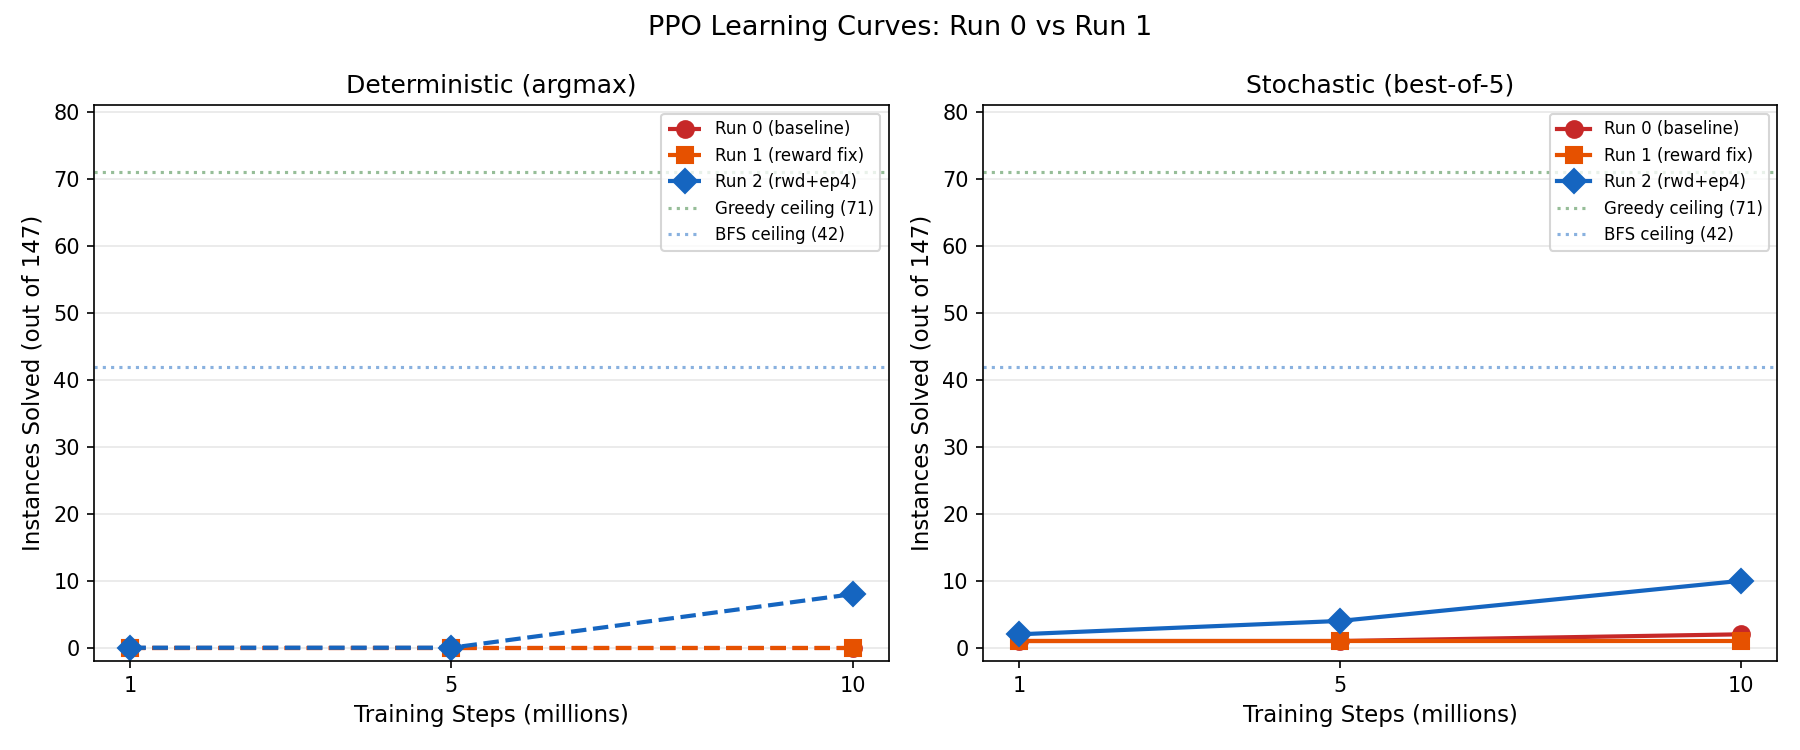
\includegraphics[width=0.95\textwidth]{figures/mini_learning_curves.png}
  \end{center}
  \vspace{-0.5em}
  \footnotesize
  PPO solve counts at 1M, 5M, 10M checkpoints (deterministic and stochastic best-of-5).\\
  Run 2 shows clear upward trajectory; Runs 0 and 1 remain near zero.\\
  {\scriptsize (Note: figure may need regeneration to include Run 2 data.)}
\end{frame}

% ──────────────────────────────────────────────────────────────────────────────
\begin{frame}{Heatmaps: Classical vs.\ PPO Solve Rates}
  \begin{center}
    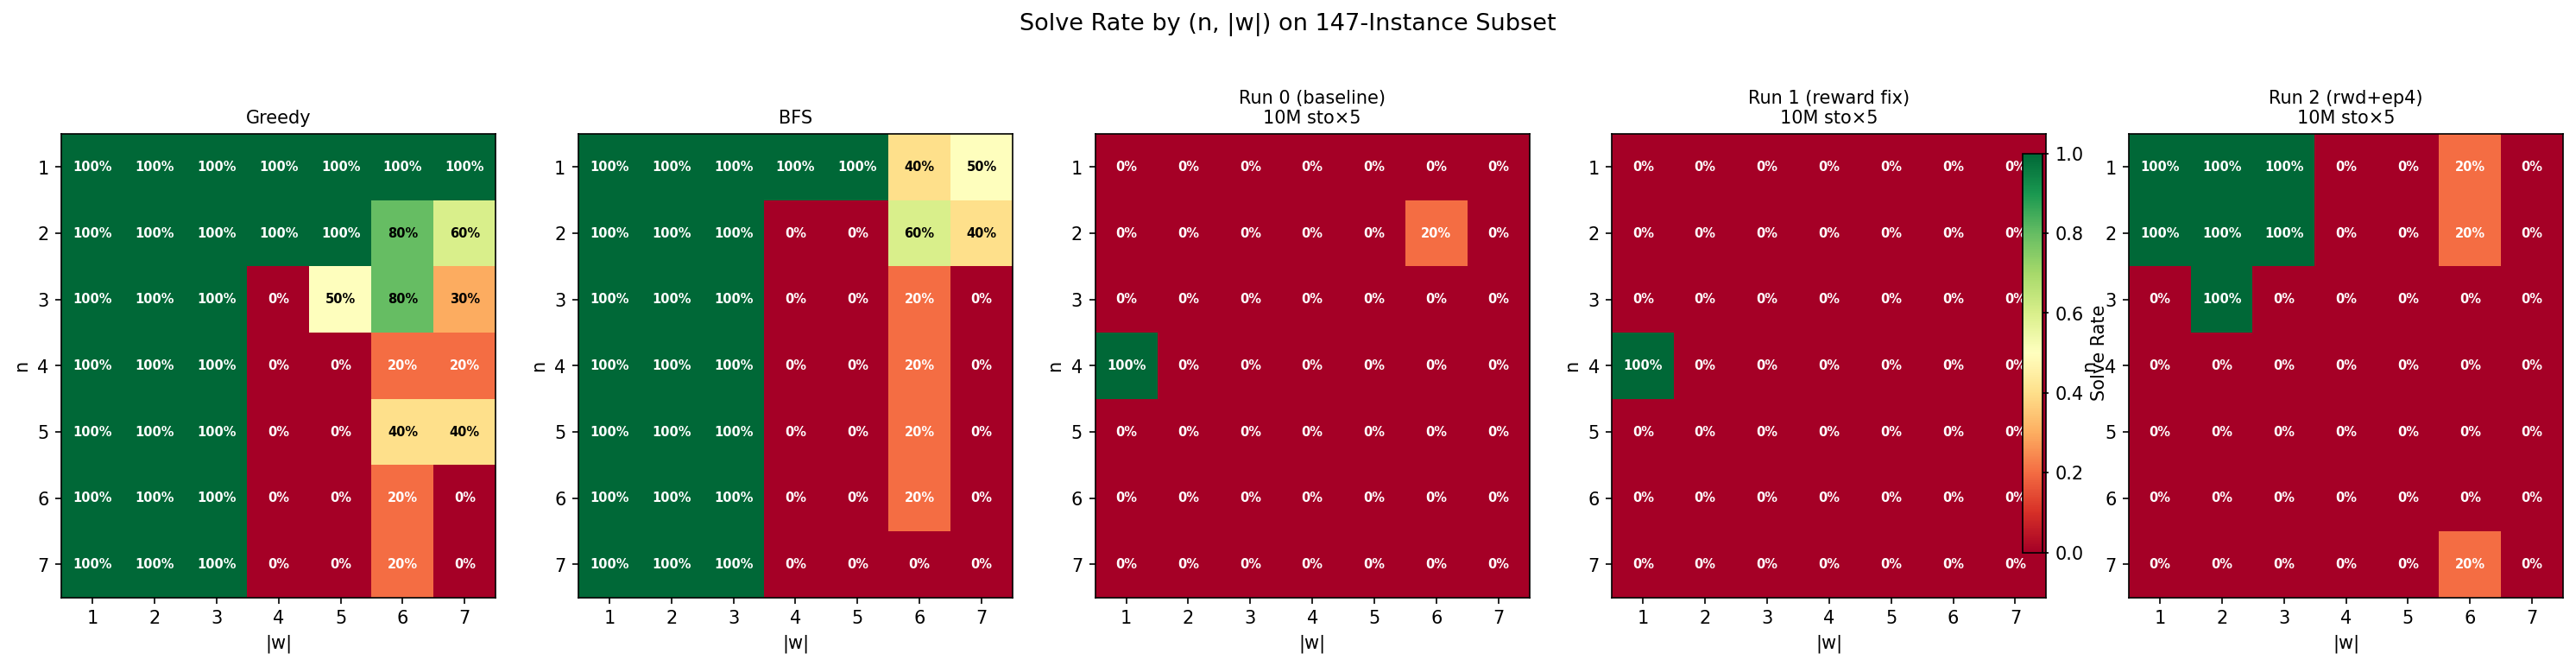
\includegraphics[width=0.95\textwidth]{figures/mini_heatmaps.png}
  \end{center}
  \vspace{-0.5em}
  \footnotesize
  Per-$(n, |w|)$ solve rates.  Greedy and BFS show clear structure.\\
  Run 2 begins to show structure at low $n$ and $|w|$.\\
  {\scriptsize (Note: figure may need regeneration to include Run 2 data.)}
\end{frame}

% ──────────────────────────────────────────────────────────────────────────────
\begin{frame}{Solve Counts: Bar Chart Overview}
  \begin{center}
    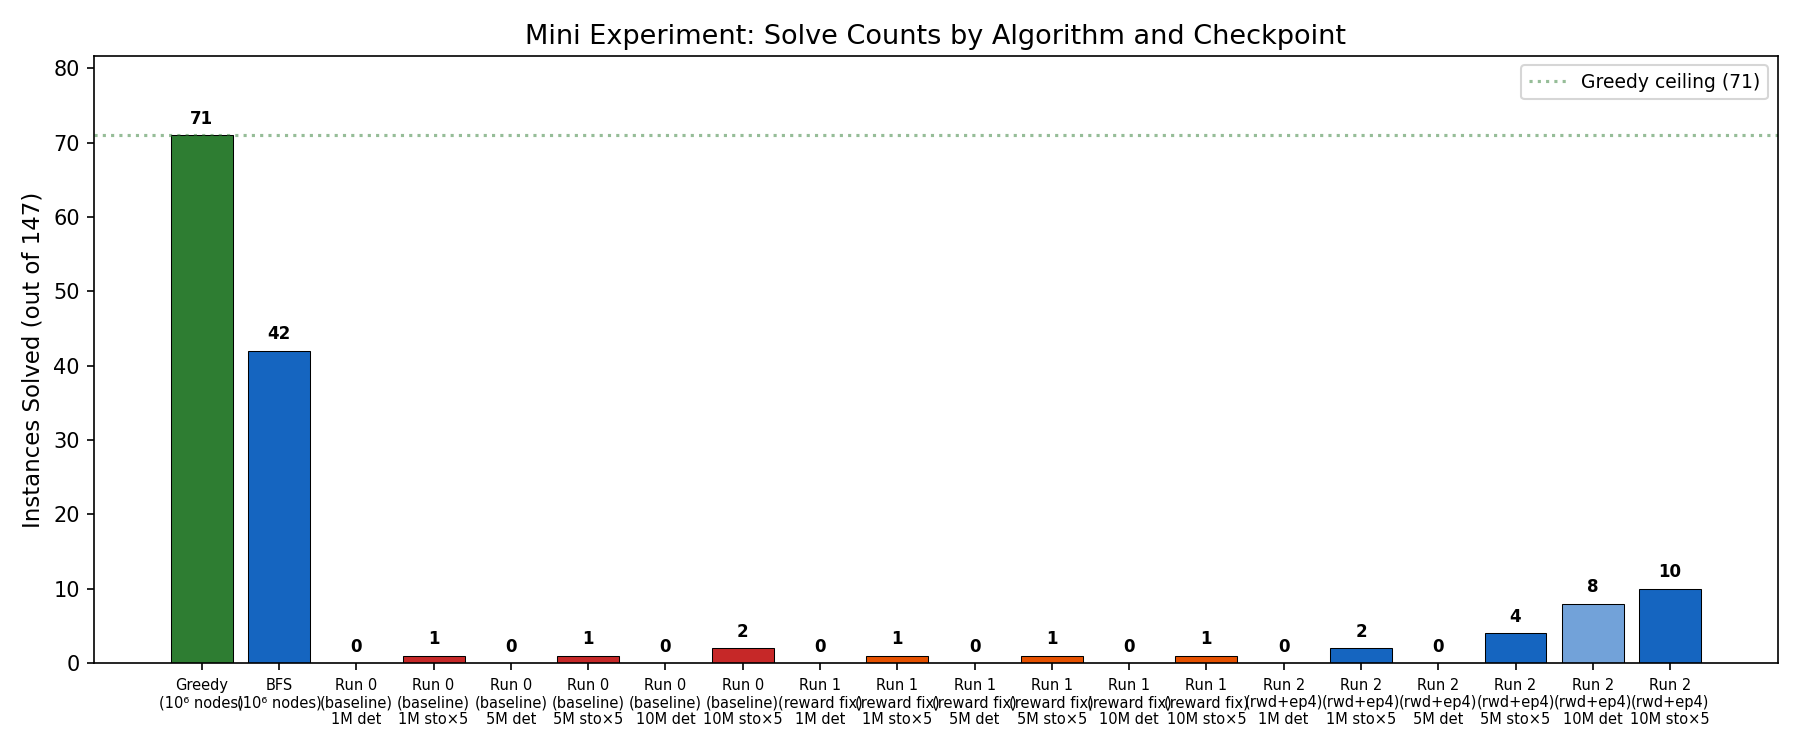
\includegraphics[width=0.95\textwidth]{figures/mini_solve_counts.png}
  \end{center}
  \vspace{-0.5em}
  \footnotesize
  All algorithms and checkpoints on the 147-instance subset.\\
  Run 2 at 10M is the first PPO configuration to show visible bars.
\end{frame}

% ──────────────────────────────────────────────────────────────────────────────
\begin{frame}{Training Solve Rate vs.\ Evaluation: A Warning}
  \small
  \begin{center}
  \begin{tabular}{lrr}
    \toprule
    & \textbf{Training ``solved''} & \textbf{Eval (sto$\times$5)} \\
    \midrule
    Run 0 at 10M & 1190 (cumulative) & \textcolor{bad}{2/147 (1.4\%)} \\
    Run 1 at 10M & 1190 (cumulative) & \textcolor{bad}{1/147 (0.7\%)} \\
    Run 2 at 10M & 1190 (cumulative) & \textcolor{good}{10/147 (6.8\%)} \\
    \midrule
    Previous 100M run & 1190/1190 & \textcolor{bad}{32/1190 (2.7\%)} \\
    \bottomrule
  \end{tabular}
  \end{center}

  \bigskip
  \textbf{Why the gap?}
  \begin{itemize}
    \item Training uses \textbf{stochastic} sampling --- a 200-step random walk often stumbles onto easy solutions
    \item ``Total solved'' is \textbf{cumulative} --- counts \emph{every} instance solved across all episodes
    \item Evaluation uses \textbf{deterministic} (argmax) or controlled stochastic rollouts
    \item Training solve rate is \alert{not a reliable performance metric}
  \end{itemize}

  \medskip
  Even Run 2's 10/147 eval rate is modest compared to training's 1190 cumulative ---
  but it is the first time eval shows a \emph{real} learned policy.
\end{frame}

% ══════════════════════════════════════════════════════════════════════════════
\section{Analysis and Next Steps}
% ══════════════════════════════════════════════════════════════════════════════

% ──────────────────────────────────────────────────────────────────────────────
\begin{frame}{Success Criteria: Results}
  \begin{center}
  \small
  \begin{tabular}{llll}
    \toprule
    \textbf{Criterion} & \textbf{Threshold} & \textbf{Actual} & \textbf{Status} \\
    \midrule
    Reward fix works   & Run 1 $> 2\times$ Run 0  & 1 vs.\ 2 (sto5) & \textcolor{bad}{Not met} \\
    Epochs help        & Run 2 $>$ Run 1 by 30\%  & 10 vs.\ 1 ($10\times$!) & \textcolor{good}{\checkmark\checkmark Met} \\
    Combined viable    & Run 2 $>$ 5/147          & 10/147            & \textcolor{good}{\checkmark Met} \\
    Approaching paper  & Run 2 $>$ 15/147 (10\%)  & 10/147 (6.8\%)    & \textcolor{neutral}{Partial} \\
    Baselines hold     & Greedy $\approx$ 46\%    & 48.3\%            & \textcolor{good}{\checkmark Met} \\
    \bottomrule
  \end{tabular}
  \end{center}

  \bigskip
  \textbf{Summary of findings:}
  \begin{enumerate}
    \item The reward fix alone is \textbf{insufficient} --- it helps the critic but
      \texttt{norm\_adv} makes the policy insensitive to reward scale.
    \item \textbf{Epochs${}=4$ is the critical fix.}  It compensates for our $3.5\times$
      smaller batch and enables the policy to actually learn.
    \item The combination (reward fix + epochs) is \textbf{viable} at 10M steps:
      8 deterministic, 10 stochastic solves --- a genuine signal worth extending.
    \item Run 2 is still scaling at 10M (monotonic improvement across checkpoints),
      suggesting more training will yield more solves.
  \end{enumerate}
\end{frame}

% ──────────────────────────────────────────────────────────────────────────────
\begin{frame}{Paper vs.\ Our Setup: The Complete Gap Analysis}
  \footnotesize
  The paper (Appendix~A) uses CleanRL with \texttt{norm\_adv=True}, separate actor/critic,
  single Adam optimiser --- \textbf{identical to our implementation}.

  \medskip
  \begin{center}
  \begin{tabular}{lrrl}
    \toprule
    \textbf{Parameter} & \textbf{Paper} & \textbf{Ours (Run 2)} & \textbf{Gap} \\
    \midrule
    \texttt{num\_envs}         & 28      & 8       & $3.5\times$ fewer \\
    \texttt{batch\_size}       & 5{,}600 & 1{,}600 & $3.5\times$ smaller \\
    \texttt{update\_epochs}    & 1       & \textcolor{good}{4} & \textcolor{good}{Compensates batch gap} \\
    Effective data/update      & 5{,}600 & \textcolor{good}{6{,}400} & \textcolor{good}{$1.14\times$ more} \\
    \texttt{total\_timesteps}  & $10^8$  & $10^7$  & $10\times$ fewer \\
    \texttt{rewards /= 14400}  & \textbf{No} & \textcolor{good}{No}  & \textcolor{good}{Fixed} \\
    \texttt{norm\_adv}         & True    & True    & Same \\
    \midrule
    \textbf{Result}            & \textcolor{good}{431/1190 (36\%)} & 10/147 (6.8\%) & Training budget \\
    \bottomrule
  \end{tabular}
  \end{center}

  \medskip
  \textbf{Remaining gap:} primarily \textbf{training budget} ($10\times$) and
  \textbf{dataset size} (147 vs.\ 1190).  The hyperparameter gaps have been closed.
\end{frame}

% ──────────────────────────────────────────────────────────────────────────────
\begin{frame}{The Learning Pipeline: Where Each Fix Acts}
  \small
  \begin{center}
  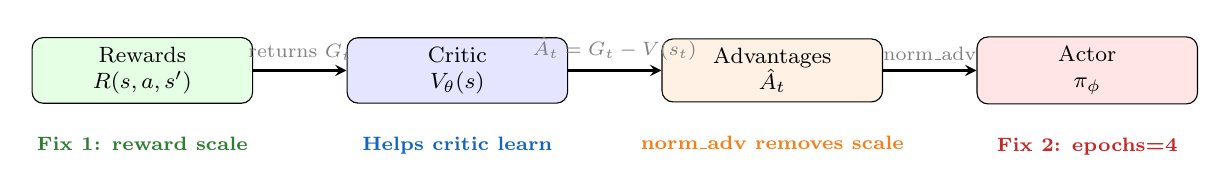
\begin{tikzpicture}[
    box/.style={draw, rounded corners, minimum height=0.8cm, minimum width=2.8cm,
                align=center, font=\footnotesize},
    arrow/.style={->, thick, >=stealth},
    label/.style={font=\scriptsize, text=gray}
  ]
    \node[box, fill=green!10] (rew) at (0,0) {Rewards\\$R(s,a,s')$};
    \node[box, fill=blue!10] (critic) at (4,0) {Critic\\$V_\theta(s)$};
    \node[box, fill=orange!10] (adv) at (8,0) {Advantages\\$\hat{A}_t$};
    \node[box, fill=red!10] (actor) at (12,0) {Actor\\$\pi_\phi$};

    \draw[arrow] (rew) -- node[above, label] {returns $G_t$} (critic);
    \draw[arrow] (critic) -- node[above, label] {$\hat{A}_t = G_t - V(s_t)$} (adv);
    \draw[arrow] (adv) -- node[above, label] {norm\_adv} (actor);

    \node[font=\scriptsize\bfseries, text=good, below=0.3cm of rew] {Fix 1: reward scale};
    \node[font=\scriptsize\bfseries, text=accent, below=0.3cm of critic] {Helps critic learn};
    \node[font=\scriptsize\bfseries, text=neutral, below=0.3cm of adv] {norm\_adv removes scale};
    \node[font=\scriptsize\bfseries, text=bad, below=0.3cm of actor] {Fix 2: epochs=4};
  \end{tikzpicture}
  \end{center}

  \bigskip
  \begin{enumerate}
    \item \textbf{Reward scale} (Fix 1) $\to$ critic can learn meaningful $V(s)$ differences
      $\to$ advantages point in the right \emph{direction}
    \item \textbf{Epochs} (Fix 2) $\to$ extract enough signal from each batch to overcome
      gradient noise $\to$ policy actually updates
    \item \textbf{Both needed:} Fix 1 without Fix 2 $=$ good advantages, but too noisy
      to use (Run 1). Fix 2 without Fix 1 $=$ not tested, but likely weak
      (critic still can't distinguish states).
  \end{enumerate}

  \smallskip
  \texttt{norm\_adv} removes advantage \emph{scale}; it cannot remove \emph{noise}.
\end{frame}

% ──────────────────────────────────────────────────────────────────────────────
\begin{frame}{Why Epochs Worked: The Complete Picture}
  \small
  \textbf{The causal chain:}

  \medskip
  \begin{enumerate}\setlength\itemsep{4pt}
    \item \textbf{Small batch} (1{,}600 vs.\ 5{,}600): each minibatch of 400 transitions
      produces a noisy gradient estimate.
    \item \textbf{epochs${}=1$}: only 4 gradient steps per PPO update.
      The noise dominates --- the policy takes a near-random walk in parameter space.
      Clipfrac $= 0$, approx\_kl $= 0$: the policy is not moving at all.
    \item \textbf{epochs${}=4$}: 16 gradient steps per PPO update.
      The noise averages out --- the policy moves in a consistent direction.
      Clipfrac $= 0.0016$: clipping activates, proving the policy is updating.
    \item \textbf{Result}: entropy drops (policy specialises), top-1 increases
      (confident actions), and eventually the policy solves 8 instances deterministically.
  \end{enumerate}

  \medskip
  \begin{block}{The Insight}
    With a small batch, the gradient SNR per step is too low for 1 epoch to extract
    meaningful signal.  Epochs${}=4$ provides the $4\times$ amplification needed to cross
    the learning threshold.  This is the single most impactful change in our ablation.
  \end{block}
\end{frame}

% ──────────────────────────────────────────────────────────────────────────────
\begin{frame}{Next Steps: Extend Run 2 to 50M Steps}
  \small
  \textbf{Why 50M:}
  \begin{itemize}
    \item Run 2 is still improving at 10M (monotonic across all checkpoints)
    \item The paper trains for $10^8$ steps --- we have used only $10^7$
    \item At 10M, Run 2 achieves 6.8\% vs.\ the paper's 36\% at $10^8$
    \item The scaling trajectory (2 $\to$ 4 $\to$ 10 sto5) suggests substantial headroom
  \end{itemize}

  \medskip
  \textbf{Recommended configuration:}
  \begin{center}
  \footnotesize
  \begin{tabular}{ll}
    \toprule
    \textbf{Parameter} & \textbf{Value} \\
    \midrule
    Base config & Run 2 (reward fix + epochs${}=4$) \\
    Total steps & 50M \\
    LR schedule & Linear$\to$0 (or cosine with floor --- test both) \\
    Checkpoints & Every 5M for evaluation curve \\
    \bottomrule
  \end{tabular}
  \end{center}

  \medskip
  \textbf{Decision rule:}
  \begin{itemize}
    \item If 50M run solves $>$20/147 (14\%): scale to full dataset (1190 instances)
    \item If 50M run solves $>$50/147 (34\%): approaching paper-level performance
    \item If 50M run plateaus $<$15/147: investigate batch size (need more envs)
  \end{itemize}
\end{frame}

% ══════════════════════════════════════════════════════════════════════════════
\appendix
% ══════════════════════════════════════════════════════════════════════════════

\begin{frame}[fragile,allowframebreaks]{Appendix: CLI Commands}
  \footnotesize
  \textbf{Classical baselines:}
  \begin{lstlisting}[language=bash]
python -m ac_solver.search.miller_schupp.evaluate \
    --search-fn greedy --max-nodes 1000000 --workers 4 --every-k 10 \
    --output results/greedy_subset_k10.csv
python -m ac_solver.search.miller_schupp.evaluate \
    --search-fn bfs --max-nodes 1000000 --workers 2 --every-k 10 \
    --output results/bfs_subset_k10.csv
  \end{lstlisting}

  \textbf{PPO training:}
  \begin{lstlisting}[language=bash]
# Run 0: baseline
python -m ac_solver.agents.ppo --preset mac --seed 1 --exp-name diag_baseline
# Run 1: reward fix
python -m ac_solver.agents.ppo --preset mac --seed 1 \
    --skip-reward-division --exp-name diag_reward_fix
# Run 2: reward fix + epochs=4
python -m ac_solver.agents.ppo --preset mac --seed 1 \
    --skip-reward-division --update-epochs 4 --exp-name diag_reward_epochs
  \end{lstlisting}
\end{frame}

% ──────────────────────────────────────────────────────────────────────────────
\begin{frame}{Appendix: Experiment File Locations}
  \small
  \begin{tabular}{ll}
    \toprule
    \textbf{Artifact} & \textbf{Path} \\
    \midrule
    Experiment spec & \texttt{spec/2026-04-03-scaled-experiment.md} \\
    \midrule
    Greedy subset CSV  & \texttt{results/greedy\_subset\_k10.csv} \\
    BFS subset CSV     & \texttt{results/bfs\_subset\_k10.csv} \\
    \midrule
    Run 0 checkpoints  & \texttt{out/diag\_baseline\_ppo-\ldots/ckpt\_*.pt} \\
    Run 0 metrics      & \texttt{results/mini\_experiment/run0\_baseline\_metrics.csv} \\
    Run 1 checkpoints  & \texttt{out/diag\_reward\_fix\_ppo-\ldots/ckpt\_*.pt} \\
    Run 1 metrics      & \texttt{results/mini\_experiment/run1\_reward\_fix\_metrics.csv} \\
    Run 2 checkpoints  & \texttt{out/diag\_reward\_epochs\_ppo-\ldots/ckpt\_*.pt} \\
    Run 2 metrics      & \texttt{results/mini\_experiment/run2\_reward\_epochs\_metrics.csv} \\
    \midrule
    This presentation  & \texttt{presentations/mini\_reproducing\_results\_slides.tex} \\
    \bottomrule
  \end{tabular}
\end{frame}

\end{document}
